\documentclass{article}
\usepackage{amsmath}
\usepackage{amsfonts}
\usepackage{graphicx}
\usepackage[final]{pdfpages}
\usepackage{hyperref}
\usepackage{mathrsfs}

\newcommand{\emptymacro}{}    % Used to test against an empty macro
\newcommand{\linearalgebra}{} 

\title{MIT Math Problems}
\author{Cecilia Chan}
\date{August 2022}

\begin{document}
\maketitle

\section*{Links}
    \begin{enumerate}
        \item \href{https://math.mit.edu/academics/undergrad/roadmaps.php}{Roadmap}
        \ifx\linearalgebra\emptymacro
        \item \href{https://ocw.mit.edu/courses/18-700-linearalgebra-fall-2013/}{Linear Algebra}
        \begin{enumerate}
            \item \hyperlink{LinearAlgebra-ProblemSet1.1}{ProblemSet1}
            \item \hyperlink{LinearAlgebra-ProblemSet2.1}{ProblemSet2}
            \item \hyperlink{LinearAlgebra-ProblemSet3.1}{ProblemSet3}
            \item \hyperlink{LinearAlgebra-ProblemSet4.1}{ProblemSet4}
            \item \hyperlink{LinearAlgebra-ProblemSet5.1}{ProblemSet5}
            \item \hyperlink{LinearAlgebra-ProblemSet6.1}{ProblemSet6}
            \item \hyperlink{LinearAlgebra-ProblemSet7.1}{ProblemSet7}
            \item \hyperlink{LinearAlgebra-ProblemSet8.1}{ProblemSet8}
            \item \hyperlink{LinearAlgebra-ProblemSet9.1}{ProblemSet9}
        \end{enumerate}
        \fi
        \item \href{https://math.mit.edu/classes/18.703/index.html}{Modern Algebra}
        \begin{enumerate}
            \item \hyperlink{ModernAlgebra-Assignment01}{Assignment1}
            \item \hyperlink{ModernAlgebra-Assignment02}{Assignment2}
            \item \hyperlink{ModernAlgebra-Assignment03}{Assignment3}
        \end{enumerate}
    \end{enumerate}

\ifx\linearalgebra\emptymacro
%
% Linear Algebra
%
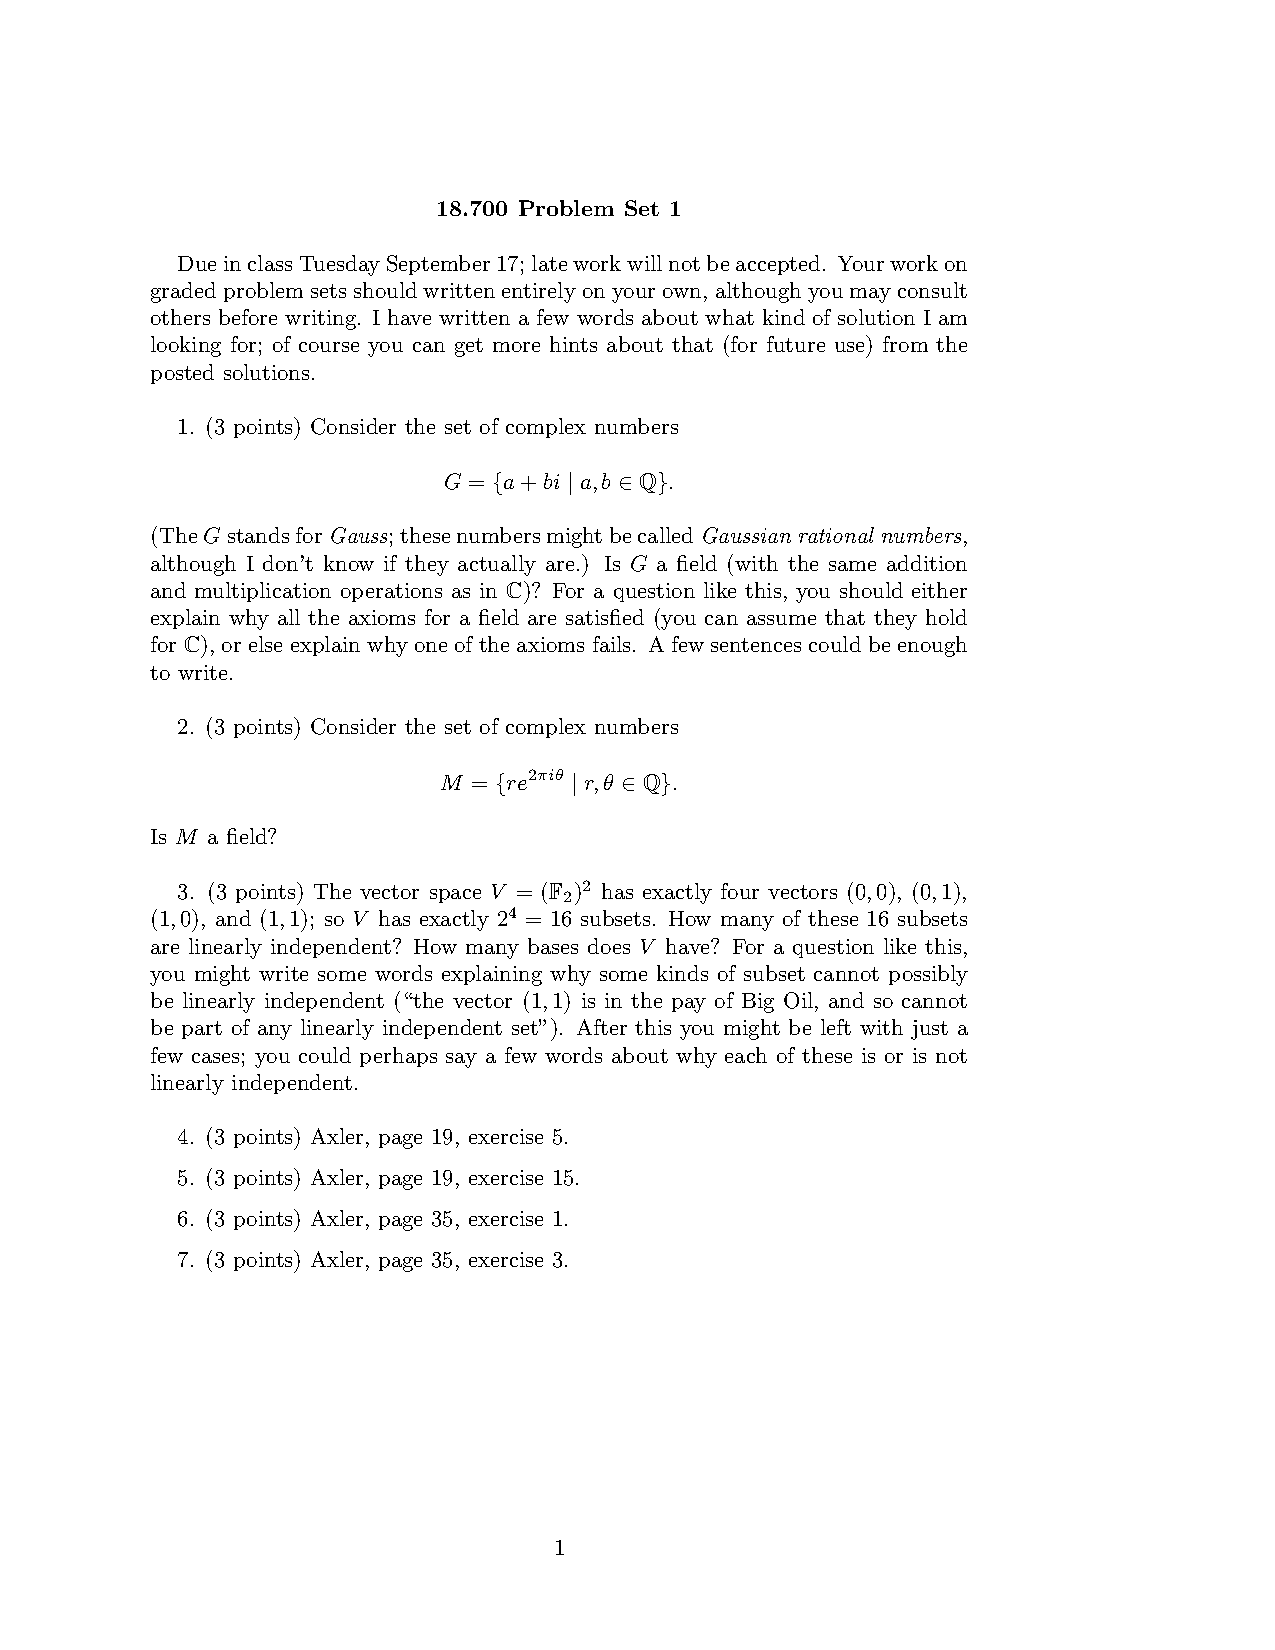
\includepdf[link=true, linkname=LinearAlgebra-ProblemSet1,pages=1]{MIT/Problems/18.700/ProblemSet1.pdf}
\section*{Question 1}
Instead of proving $ G $ is a field directly, it is easier to observe that $ G $ is a subset of $ C $, and so we can prove that $ G $ is a field by proving this lemma first:

If $ H $ is a subset of a field $ F $, then $ H $ is a field (inheriting the operations from $ F $) if 
\begin{enumerate}
    \item There exists an element $ h \ne 0 \in H $, 
    \item for all $ p, q \in H $, $ p - q \in H $, and
    \item for all $ p, q \ne 0 \in H $, $ \frac{p}{q} \in H $.
\end{enumerate}

By setting $ p = q = h $, using the rule 2 and 3, we get that $ 0 \in H $ and $ 1 \in H $. By setting $ p = 0 $, using rule 2, we get that additive inverse exists in $ H $. By setting $ p = 1 $, using rule 3, we get that multiplicative inverse exists in $ H $. Using inverses, we know sum and product exists in $ H $. All other field axioms simply inherits from $ F $, therefore $ H $ is a field.

With the lemma, in order to prove that $ G $ is a field. It suffice to show the three conditions. 

\begin{enumerate}
    \item we have  $ 1 + 0i \in H $, 
    \item for any $ (a + bi), (c + di) \in G $, we have $ (a + bi) - (c + di) = (a-c) + (b-d)i \in G $. 
    \item for any $ (a + bi), (c + di) \in G $, we have $ \frac{a + bi}{c + di} = \frac{(a+bi)(c-di)}{c^2 + d^2} = \frac{ac+bd}{c^2+d^2} + \frac{bc-ad}{c^2+d^2}i \in G $.
\end{enumerate}

Therefore we conclude $ G $ is a field.
\section*{Question 2}
$ M $ is not a field because $ e^{2 \pi i \left(\frac{1}{4}\right)} + e^{2 \pi i (0)} = i + 1 = \sqrt{2} e^{2 \pi i \frac{1}{8} i} \notin M $
\section*{Question 3}
To start with, $ (0, 0) $ cannot be part of a basis, so we are left with 3 vectors.

Obviously, $ \{(1, 0), (0, 1)\} $ is a basis, so we know the dimension of the vector space is 2.

All $ \left( \begin{array}{c} 3 \\ 2 \end{array} \right) $ subsets of vector is a basis, because of the following:

\begin{eqnarray*}
\left|
\begin{array}{cc}
  1 & 0 \\
  0 & 1
\end{array}
\right| &=& 1 \\
\left|
\begin{array}{cc}
  1 & 1 \\
  0 & 1
\end{array}
\right| &=& 1 \\
\left|
\begin{array}{cc}
  0 & 1 \\
  1 & 1
\end{array}
\right| &=& 1
\end{eqnarray*}
As a reminder, if the determinant is non-zero, that means an inverse exists. That inverse can be used to construct linear combinations of the vectors so that they construct the standard basis. That's why the vectors span the whole space.
\section*{Question 4}
Note that $ F^3 $ stands for either $ R^3 $ or $ C^3 $ in the book.
\subsection*{Part a}
It is a vector space because:
\begin{enumerate}
    \item {$ (0, 0, 0) $ is in the subset}
    \item { If $ a + 2b + 3c = 0 $ and $ d + 2e + 3f = 0 $, then $ (a + d) + 2(b + e) + 3 (c + f) = 0 $. Therefore, whenever $ (a,b,c) $ and $ (d,e,f) $ belongs to the subset, then $ (a,b,c) + (d,e,f) = ((a+d),(b+e),(c+f)) $ belongs to the subset too, which means the space is closed under addition.}
    \item { If $ a + 2b + 3c = 0 $ then $ (fa) + 2(fb) + 3(fc) = 0 $. Therefore, whenever $ (a,b,c) $ belongs to the subset, then $ f(a, b, c) = (fa, fb, fc) $ belongs to the subset too, which means the space is closed under scalar multiplication.}
\end{enumerate}

\subsection*{Part b}
The vector $ (0, 0, 0) $ does not belong to the subset and therefore it is not a subspace.

\subsection*{Part c}
The vector $ (1, 1, 0) $ and $ (0, 0, 1) $ belongs to the subset but their sum $ (1, 1, 1) $ is not, therefore it is not a subspace.

\subsection*{Part d}
It is a vector space because:
\begin{enumerate}
    \item {$ (0, 0, 0) $ is in the subset}
    \item { If $ a = 5c $ and $ d = 5f $, then $ (a + d) = 5(c + f) $. Therefore, whenever $ (a,b,c) $ and $ (d,e,f) $ belongs to the subset, then $ (a,b,c) + (d,e,f) = ((a+d),(b+e),(c+f)) $ belongs to the subset too, which means the space is closed under addition.}
    \item { If $ a = 5c $ then $ (fa) = 5(fc) $. Therefore, whenever $ (a,b,c) $ belongs to the subset, then $ f(a, b, c) = (fa, fb, fc) $ belongs to the subset too, which means the space is closed under scalar multiplication.}
\end{enumerate}

Apparently, this proof is the same as part a. In fact, it follows that a set of vectors satisfying a system of homogeneous linear equations (i.e. with 0 constant terms) is a subspace, and the proof is going to be identical. 
\section*{Question 5}
I have spent some time (an hour maybe) trying to prove that $ U_1 = U_2 $, but turn out that is wasted effort because $ U_1 \ne U_2 $.

As a counter example, consider:
\begin{enumerate}
  \item {$ U_1 $ to be the vector space spanned by the vectors $ \{ (1, 0) \} $.}
  \item {$ U_2 $ to be the vector space spanned by the vectors $ \{ (1, 1) \} $.}
  \item {$ W $ to be the vector space spanned by the vectors $ \{ (0, 1) \} $.}
  \item {$ V $ to be $ F^2 $.}
\end{enumerate}
\section*{Question 6}
To prove that the new set of vectors spans all the vectors spanned by the old set. One must prove that for all vectors spanned in the old set, it can be spanned by the new set. Solving that problem directly is difficult, let's us consider in general what can the new set of vector span by considering the general linear combination of the new set as follows:

\begin{eqnarray*}
  & & d_1 (v_1 - v_2) + d_2 (v_2 - v_3) + \cdots + d_{n-1}(v_{n-1} - v_n) + d_n v_n \\
  &=& d_1 v_1 - d_ 1 v_2 + d_2 v_2 - d_2 v_3 + \cdots + d_{n-1} v_{n-1} - d_{n-1} v_n + d_n v_n \\
  &=& d_1 v_1 + (d_2 - d_1) v_2 + (d_3 - d_2) v_3 + \cdots + (d_n - d_{n-1}) v_n \\
  &=& c_1 v_1 + c_2 v_2 + \cdots + c_n v_n
\end{eqnarray*}

If we read it backwards, the idea is that if we could find $ d_i $ in terms of $ c_i $, then we solved the problem. It is obvious that $ d_1 = c_1 $, and also, for all $i \ge 2 $, $ d_i - d_{i-1} = c_i $. A simple manipulation yield the recurrence relation $ d_i = d_{i-1} + c_i $, which gives $ d_i = \sum\limits_{k=1}^{i}{c_k} $. That solved our problem!

To present this formally, we prove that 
\begin{eqnarray*}
  & & d_1 (v_1 - v_2) + d_2 (v_2 - v_3) + \cdots + d_{n-1}(v_{n-1} - v_n) + d_n v_n \\
  &=& \sum\limits_{i=1}^{n-1} d_i (v_i - v_{i+1}) + d_n v_n \\
  &=& \sum\limits_{i=1}^{n-1} d_i v_i - \sum\limits_{i=1}^{n-1} d_i v_{i+1} + d_n v_n \\
  &=& \sum\limits_{i=1}^{n-1} \sum\limits_{k=1}^{i}{c_k} v_i - \sum\limits_{i=1}^{n-1} \sum\limits_{k=1}^{i}{c_k} v_{i+1} + \sum\limits_{k=1}^{n}{c_k} v_n \\
  &=& \sum\limits_{i=1}^{n-1} \sum\limits_{k=1}^{i}{c_k} v_i - \sum\limits_{i=2}^{n} \sum\limits_{k=1}^{i-1}{c_k} v_{i} + \sum\limits_{k=1}^{n}{c_k} v_n \\
  &=& c_1 v_1 + \sum\limits_{i=2}^{n-1} \sum\limits_{k=1}^{i}{c_k} v_i - \sum\limits_{i=2}^{n} \sum\limits_{k=1}^{i-1}{c_k} v_{i} + \sum\limits_{k=1}^{n}{c_k} v_n \\
  &=& c_1 v_1 + \sum\limits_{i=2}^{n-1} \left(\sum\limits_{k=1}^{i-1}{c_k} v_i + c_iv_i\right) - \sum\limits_{i=2}^{n} \sum\limits_{k=1}^{i-1}{c_k} v_{i} + \sum\limits_{k=1}^{n}{c_k} v_n \\
  &=& c_1 v_1 + \sum\limits_{i=2}^{n-1} \sum\limits_{k=1}^{i-1}{c_k} v_i + \sum\limits_{i=2}^{n-1} c_iv_i - \sum\limits_{i=2}^{n} \sum\limits_{k=1}^{i-1}{c_k} v_{i} + \sum\limits_{k=1}^{n}{c_k} v_n \\
  &=& c_1 v_1 + \sum\limits_{i=2}^{n-1} \sum\limits_{k=1}^{i-1}{c_k} v_i + \sum\limits_{i=2}^{n-1} c_iv_i - \sum\limits_{i=2}^{n-1} \sum\limits_{k=1}^{i-1}{c_k} v_{i} - \sum\limits_{k=1}^{n-1}{c_k} v_n + \sum\limits_{k=1}^{n}{c_k} v_n \\
  &=& c_1 v_1 + \sum\limits_{i=2}^{n-1} c_iv_i - \sum\limits_{k=1}^{n-1}{c_k} v_n + \sum\limits_{k=1}^{n}{c_k} v_n \\
  &=& c_1 v_1 + \sum\limits_{i=2}^{n-1} c_iv_i + c_n v_n \\
  &=& c_1 v_1 + c_2 v_2 + \cdots + c_n v_n
\end{eqnarray*}

The manipulation is tedious and obscure the original idea, that's why I wrote the above before the formal presentation. The key trick is to arrange the two big double summations introduced in line 4 to cancel each other. Most steps after line 4 is just to make sure all the indices matches up so that we can cancel. We knew that's the answer, so any terms that left will form exactly the linear combination we need.
\section*{Question 7}
Since $ \{v_1 + w, v_2 + w, \cdots v_n + w \}$ is linearly dependent, there exists $ c_i $ not all zero such that $ \sum\limits_{i=1}^{n} c_i(v_i + w) = 0 $. A simple manipulation shows that $ \left(\sum\limits_{i=1}^{n} c_i \right) w = \sum\limits_{i=1}^{n} -c_i v_i $.

Suppose (for the sake of contradiction) that $ D = \sum\limits_{i=1}^{n} c_i = 0 $, then the left hand side of the equation is 0 and we have found a non-trivial linear combination of $ v_i $ that sums to zero, contradicting the fact the $ \{v_1, v_2, \cdots, v_n \} $ is linearly independent. Therefore $ D \ne 0 $, and $ w = \sum\limits_{i=1}^{n} -\frac{c_i}{D} v_i $ so $ w \in span(\{v_1, v_2, \cdots, v_n \}) $.

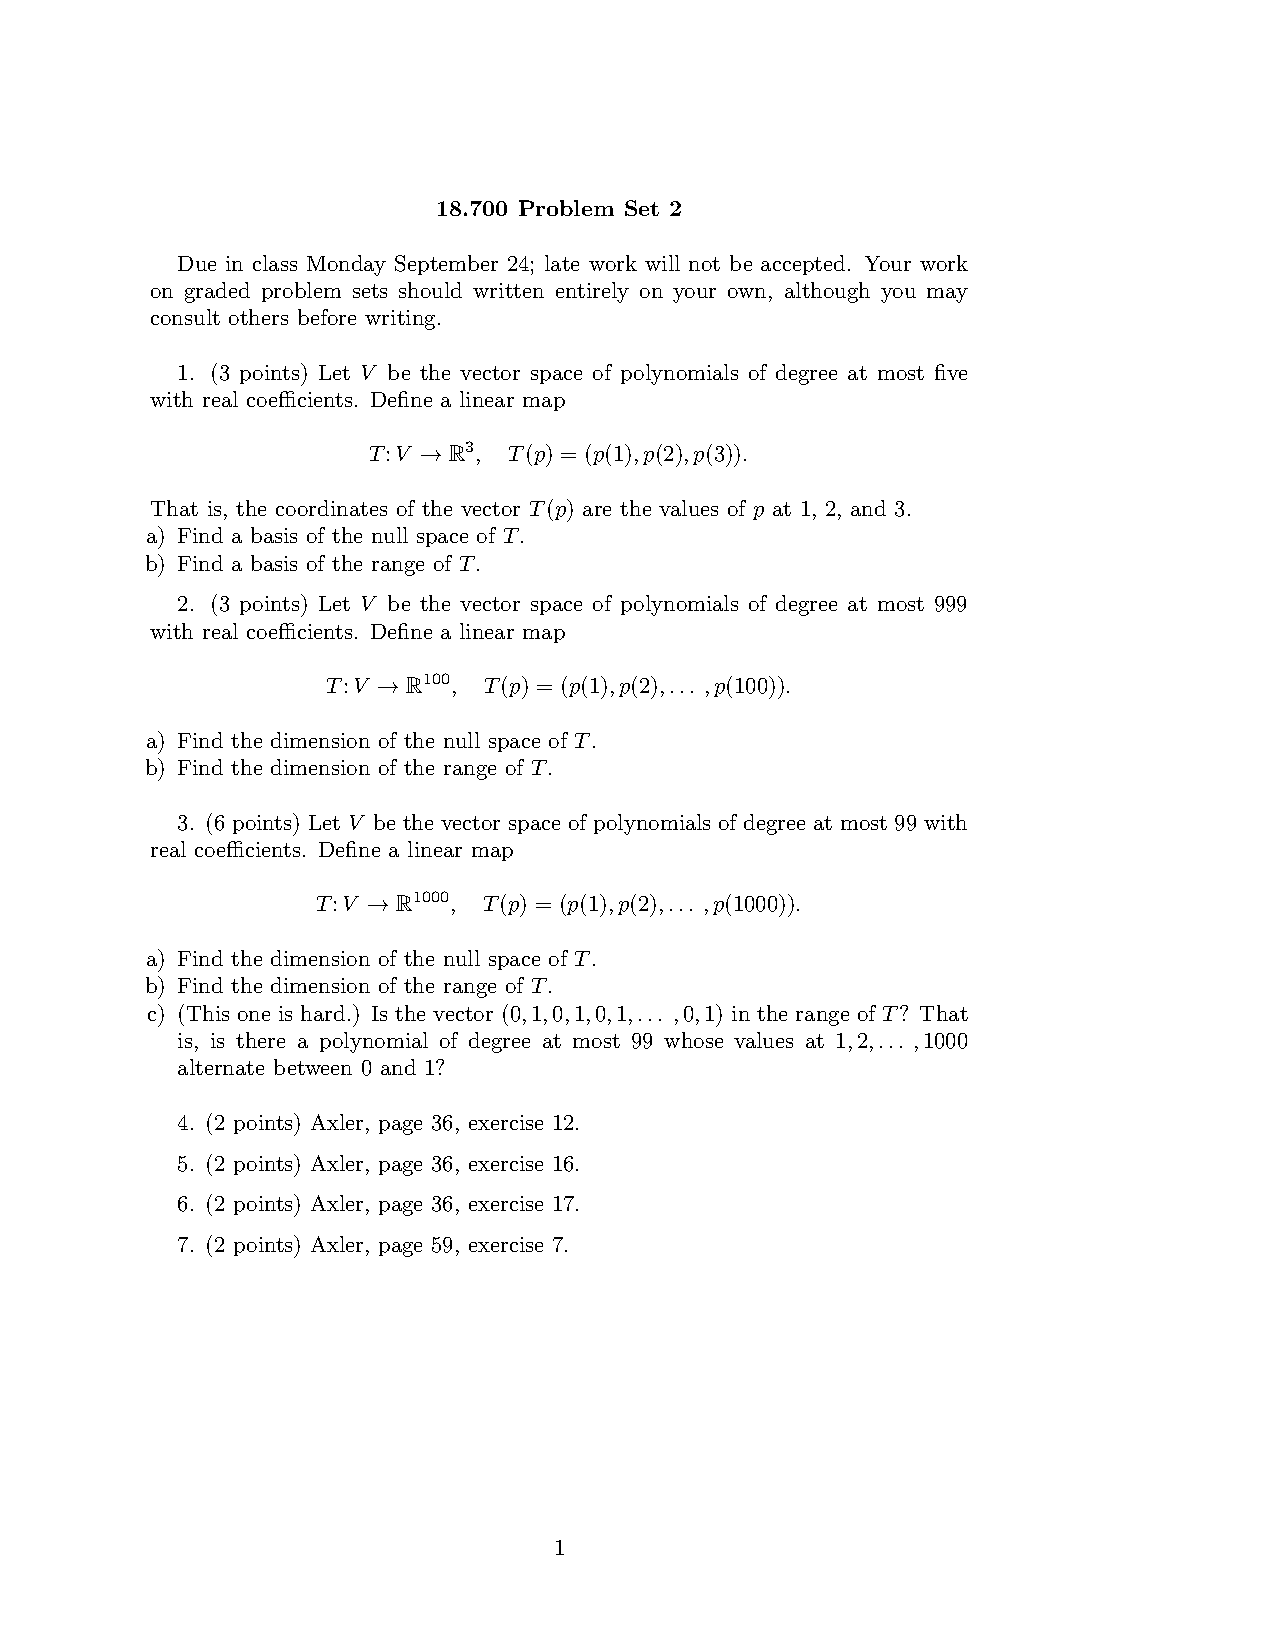
\includepdf[link=true, linkname=LinearAlgebra-ProblemSet2,pages=1]{MIT/Problems/18.700/ProblemSet2.pdf}
\section*{Question 1}
\subsection*{Part a}
The null space $ ker(T) $ of the linear transformation $ T $ is precisely the set of polynomials $ f $ of degree at most 5, such that $ f(1) = f(2) = f(3) = 0 $. Obviously, all such polynomial must have a factor of $ (x - 1)(x - 2)(x - 3) $. 

To simplify, let's consider the mapping $ M : ker(T) \mapsto U, M(p) = \frac{p}{(x - 1)(x - 2)(x - 3)} $

Denote $ U' $ to be the set of all polynomials with real coefficients of degree at most 2.

$ U \subset U' $ because any polynomial in $ ker(T) $ must have a factor of $ (x - 1)(x - 2)(x - 3) $ and of degree at most 5, so $ M(p) $ must be a polynomial with real coefficients with degree at most 2.

$ U' \subset U $ because when $ q \in U' $, $ f = q(x - 1)(x - 2)(x - 3) $ is a polynomial with real coefficients with degree at most 5 and $ f(1) = f(2) = f(3) = 0 $, that implies $ f \in ker(T) $ and so $ q \in U $

So $ U = U' $, but not only that, it is a vector space isomorphism because the mapping is bijective and it respects the add and scalar multiply operations.

$ U' $ has a very simple basis of $ B' = \{1, x, x^2 \} $, therefore, a basis of $ ker(T) $ is $ B = M^{-1}(B') = \{(x - 1)(x - 2)(x - 3), x(x - 1)(x - 2)(x - 3), x^2(x - 1)(x - 2)(x - 3) \} $.

\subsection*{Part b}
Using Lagrange's interpolation, for any $ (a,b,c) \in R^3 $, we can create polynomials in real coefficients that satisfy $ p(1) = a, p(2) = b, p(3) = c $ as follows:

$ \frac{(x-2)(x-3)}{(1-2)(1-3)}a + \frac{(x-1)(x-3)}{(2-2)(2-3)}b + \frac{(x-1)(x-2)}{(3-1)(3-2)}c $

That means $ Im(T) = R^3 $, which means we have a very simple basis for $ Im(T) = \{(1,0,0), (0,1,0), (0,0,1) \} $.
\section*{Question 2}
\subsection*{Part a}
Using the same trick as in question 1, $ ker(T) $ is isomorphic to the space of polynomials with real coefficients of degree at most $ 899 $, therefore the dimension of $ ker(T) $ is 899. 

\subsection*{Part b}

Using the same trick as in question 1, $ Im(T) $ is isomorphic to $ R^{100} $, therefore the dimension of $ Im(T) $ is 100.
\section*{Question 3}
\subsection*{Part a}
The only polynomial of degree at most 99 having 1000 zeros is $ f(x) = 0 $. Therefore the dimension of $ Ker(T) $ is 0.
\subsection*{Part b}
By the rank nullity theorem, $ dim(Ker(T)) + dim(Im(T)) = dim(V) $ where $ V $ is the domain of the linear transformation $ T $. Therefore the dimension of $ Im(T) $ is 100.
\subsection*{Part c}
The only polynomial of degree at most 99 having 500 zeros is $ f(x) = 0 $. But then $ f(2) = 0 \ne 1 $, therefore such a polynomial does not exist and $ (0,1,\cdots,0,1) \notin Im(T) $.
\section*{Question 4}
Since $ p_j(2) = 0 $, $ (x-2) $ is a factor of $ p_j $ for all $ j $. Consider the polynomials $ q_j = \frac{p_j}{x-2} $. These are $ m + 1 $ polynomials of degree at most $ m - 1 $, these must be linearly dependent because $ dim(p_{m-1}) = m $. So there exists a non-trivial linear combination $ \sum\limits_{i=0}^{m} c_i q_i = 0 $. Multiply by $ (x - 2) $, we have got a non-trivial linear combination $ \sum\limits_{i=0}^{m} c_i p_i = 0 $ so that these vectors are not linearly independent.
\section*{Question 5}
Since $ U_1, U_2 \cdots U_m $ are vector spaces, there exists $ B_1, B_2 \cdots B_n $ bases for them. Any vectors in $ U_1 + U_2 + \cdots + U_n $ can be written a a sum of vectors $ u_1 + u_2 + \cdots + u_n $, which can in turn written into the sum of linear combination of these basis vectors. That means $ B_1 \cup B_2 \cup \cdots \cup B_n $ spans $ U_1 + U_2 + \cdots + U_n $. The dimension is always at most the size of a spanning set, so:

\begin{eqnarray*}
    &   & dim(U_1 + U_2 + \cdots + U_n) \\
    &\le& | B_1 \cup B_2 \cup \cdots \cup B_n | \\
    &\le& | B_1 | + | B_2 | + \cdots + | B_n | \\
    &=  & dim(U_1) + dim(U_2) + \cdots + dim(U_n)
  \end{eqnarray*}
\section*{Question 6}
Using the same idea as in question 5, except we claim that the generated spanning set is actually a basis.

Suppose (for the sake of contradiction) that the spanning set is not linearly independent, then there exists a non-trivial linear combination. 

\begin{eqnarray*}
    w_1 b_1 + w_2 b_2 + \cdots w_k b_k = 0
\end{eqnarray*}

Furthermore, we can enforce some more conditions. First, $ w_j \ne 0 $ for all $ j $, this can be easily done by dropping the zero terms. Second, this sum must involve basis vectors coming from more than one vector space. This must be true because otherwise we contradict the fact that the vectors selected is a basis.

Without loss of generality, we assume $ U_1 $ is involved in the sum, and we split the sum as follow:

\begin{eqnarray*}
    (w_{11} p_1 + w_{12} p_2 + \cdots w_{1k_1} p_{k_1}) + (w_{21} q_1 + w_{22} q_2 + \cdots w_{k_2} q_{k_2}) = 0
\end{eqnarray*}

Where $ p_j $ comes from $ U_1 $ and $ q_j $ does not come from $ U_1 $.

Now it is clear that the first part of the sum is simply a vector (which we will call $ p $) in $ U_1 $, and we have found a linear combination of it by combining vectors in some other vector spaces.

Now we have found our contradiction. $ p $ can be represented as either $ p $ or the linear combination we have just found, contradicting the fact that the combined vector space is a direct sum, which requires all vectors in it have a unique representation as a sum of individual vector spaces.
\section*{Question 7}
As $ T $ is surjective, for any vector $ t $ in $ V $, there exists a vector $ v \in V $ such that $ T(v) = t $. Now $ v $ can be represented as a linear combination of the basis vector of $ V $ and $ T $ is linear, so we can apply $ T $ to both sides and so $ T(v_1) T(v_2) \cdots T(v_n) $ span $ W $.

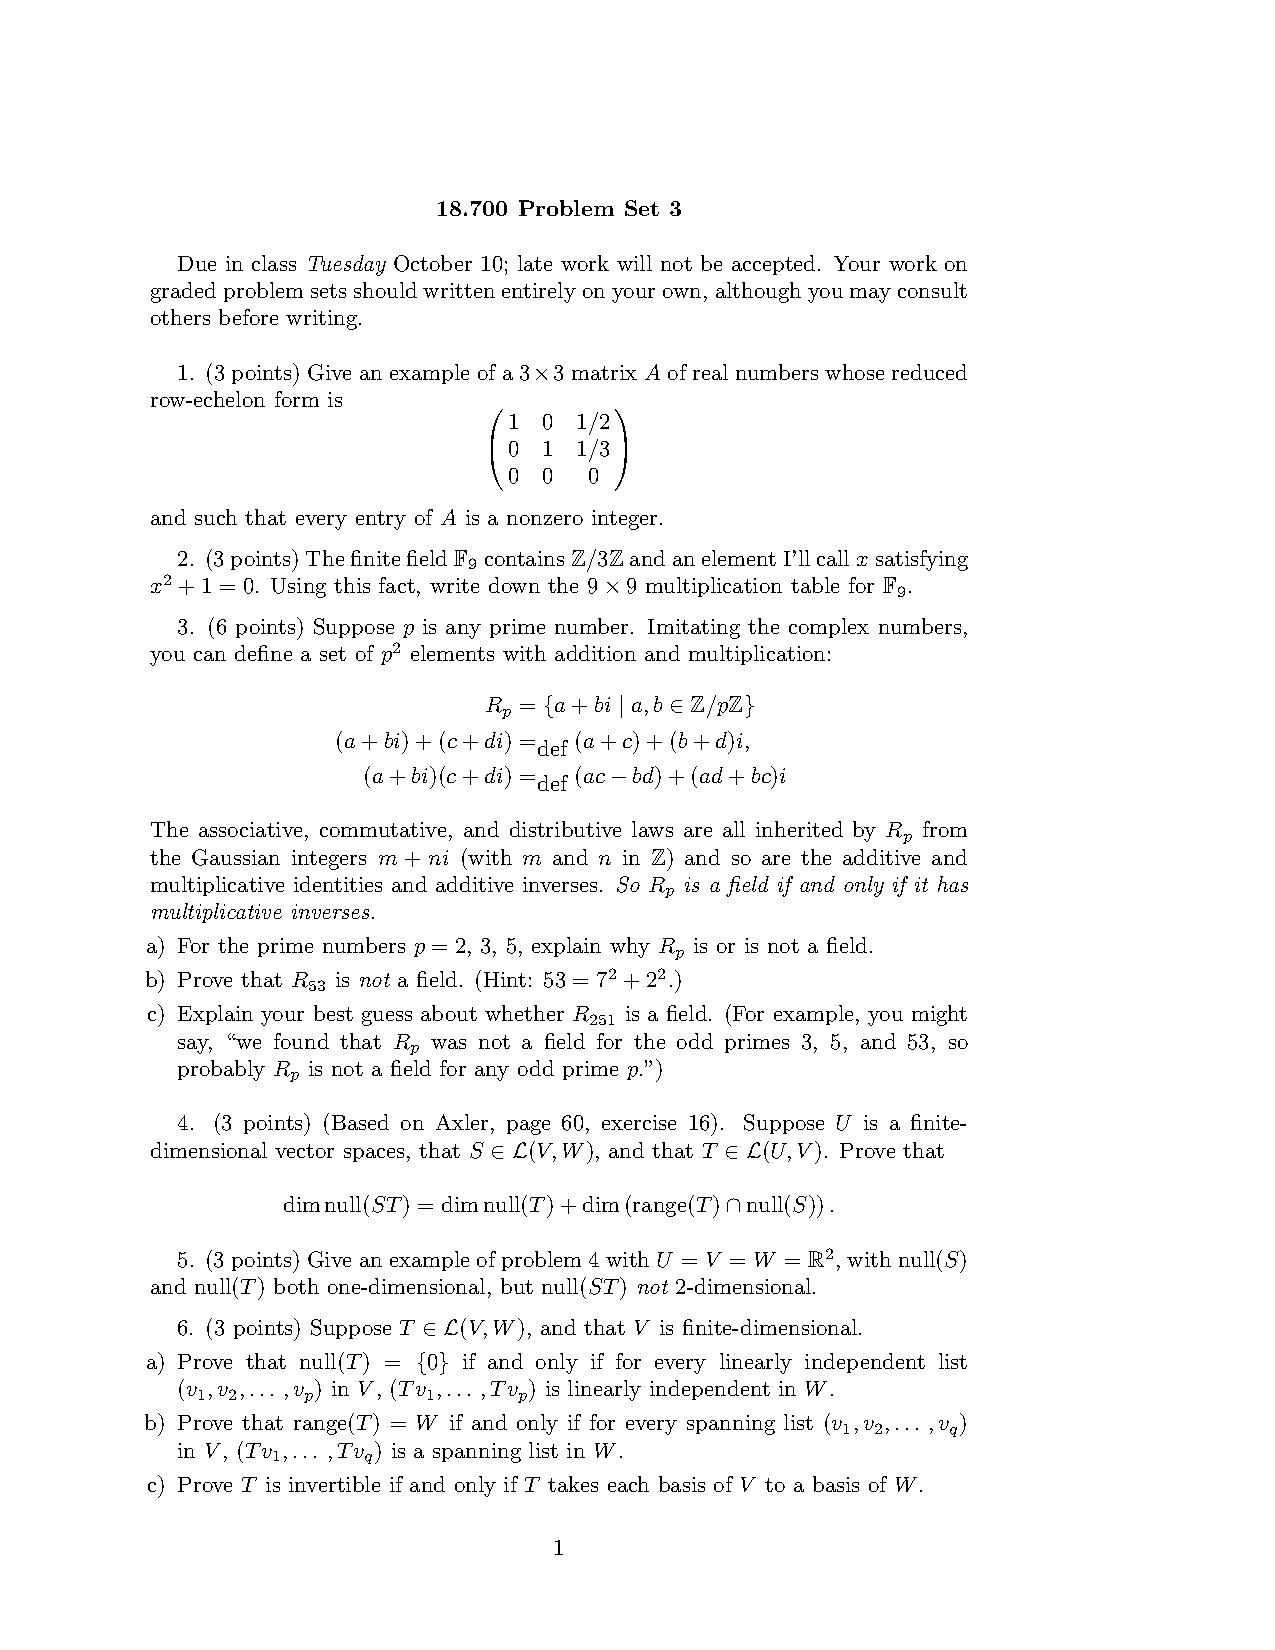
\includepdf[link=true, linkname=LinearAlgebra-ProblemSet3,pages=1]{MIT/Problems/18.700/ProblemSet3.pdf}
\section*{Question 1}
\begin{eqnarray*}
  & & \left(
        \begin{array}{ccc}
          1 & 0 & \frac{1}{2} \\
          0 & 1 & \frac{1}{3} \\
          0 & 0 & 0 
        \end{array}
      \right) \\
  & \to &
    \left(
        \begin{array}{ccc}
          2 & 0 & 1 \\
          0 & 3 & 1 \\
          0 & 0 & 0 
        \end{array}
    \right) \\
  & \to &
    \left(
        \begin{array}{ccc}
          2 & 3 & 2 \\
          0 & 3 & 1 \\
          0 & 0 & 0 
        \end{array}
    \right) \\
  & \to &
    \left(
        \begin{array}{ccc}
          2 & 3 & 2 \\
          2 & 6 & 3 \\
          0 & 0 & 0 
        \end{array}
    \right) \\       
  & \to &
    \left(
        \begin{array}{ccc}
          2 & 3 & 2 \\
          2 & 6 & 3 \\
          2 & 6 & 3
        \end{array}
    \right) \\           
\end{eqnarray*}

\section*{Question 2}
The key idea is that the $ F_9 $ elements are $ 0, 1, 2, x, x + 1, x + 2, 2x, 2x + 1 $ and $ 2x + 2$. Once we have that, the rest is simply doing all the 9 x 9 multiplication. Here are the results:
\begin{eqnarray*}
  & & \left(
        \begin{array}{ccccccccc}
0 & 0 & 0 & 0 & 0 & 0 & 0 & 0 & 0 \\
0 & 1 & 2 & x & x + 1 & x + 2 & 2x & 2x + 1 & 2x + 2 \\
0 & 2 & 1 & 2x & 2x + 2 & 2x + 1 & x & x + 2 & x + 1 \\
0 & x & 2x & 2 & x + 2 & 2x + 2 & 1 & x + 1 & 2x + 1 \\
0 & x + 1 & 2x + 2 & x + 2 & 2x & 1 & 2x + 1 & 2 & x \\
0 & x + 2 & 2x + 1 & 2x + 2 & 1 & x & x + 1 & 2x & 2 \\
0 & 2x & x & 1 & 2x + 1 & x + 1 & 2 & 2x + 2 & x + 2 \\
0 & 2x + 1 & x + 2 & x + 1 & 2 & 2x & 2x + 2 & x & 1 \\
0 & 2x + 2 & x + 1 & 2x + 1 & x & 2 & x + 2 & 1 & 2x \\
        \end{array}
      \right) \\
\end{eqnarray*}

Of course, I am not going to do that 81 multiplications myself, the work is done by these simple python code:

\begin{verbatim}
e = []

def mul(x,y):
    (a,b) = x
    (c,d) = y
    # (ax + b)(cx + d)
    # = acx^2 + (ad + bc)x + bd
    # = (ad + bc)x + (bd - ac)
    p = (a * d + b * c) % 3
    q = (b * d - a * c + 3) % 3
    if (p == 0):
        return q
    elif p == 1:
        if q == 0:
            return "x"
        else:
            return "x + %s" % q
    else:
        if q == 0:
            return "2x"
        else:
            return "2x + %s" % q

for c in range(0, 3):
    for d in range(0, 3):
        e.append((c,d))

for p in e:
    for q in e:
        print(mul(p,q),end=" ")
    print()

\end{verbatim}
\section*{Question 3}
Consider the multiplicative inverse of a general element of $ (a + bi) $ 

\begin{eqnarray*}
  & & \frac{1}{a + bi} \\
  &=& \frac{a - bi}{a^2 + b^2} \\
\end{eqnarray*}

Now since $ a, b \in Z/pZ $ which is a field, so as long as $ a^2 + b^2 \ne 0 $, the multiplicative inverse of $ a^2 + b^2 $ exists and therefore the multiplicative inverse of $ a^2 + b^2 $ exists.

To be continued
\section*{Question 4}
First, $ null(T) $ is a vector space and therefore has a basis $ t_1, t_2, ..., t_m \in U $. Also, $ null(S) $ and $ range(T) $ are vector spaces, so $ null(S) \cap range(T) $ is also a vector space and therefore has a basis $ v_1, v_2, \cdots v_n $. Each of these $ n $ vectors must have a preimage $ u_1, u_2, \cdots u_n \in U $ such that $ T(u_i) = v_i $. I claim that $ B = \{ t_1, t_2, ..., t_m, u_1, u_2, \cdots u_n \} $ is a basis for $ null(ST) $.

To show that the $ B $ spans $ null(ST) $, consider a general vector $ v \in null(ST) $. $ T(v) \in null(S) \cap range(T) $, so it can be written as a unique linear combination $ T(v) = \sum c_i v_i $. Consider: 

\begin{eqnarray*}
  & & T(v - \sum c_i u_i) \\
  &=& T(v) - \sum c_i T(u_i) \\
  &=& T(v) - \sum c_i v_i \\
  &=& T(v) - T(v) \\
  &=& 0 
\end{eqnarray*}

That means $ (v - \sum c_i u_i) \in null(T) $ and therefore:

\begin{eqnarray*}
  v - \sum c_i u_i &=& \sum d_i t_i \\
                 v &=& \sum c_i u_i + \sum d_i t_i 
\end{eqnarray*}

So $ B $ spans $ null(ST) $.

To show that $ B $ is linearly independent, suppose (for the sake of contradiction) there exists a non-trivial linear combination $ \sum c_i u_i + \sum d_i t_i = 0 $. Suppose $ c_i = 0 $ for all $ i $, we have a non-trivial linear combination $ \sum d_i t_i = 0 $, contradicting the fact that $ t_i $ is a basis of $ null(T) $. Therefore, there must be an $ c_i \ne 0 $. Applying $ T $ on the linear combination, we get 

\begin{eqnarray*}
     \sum c_i u_i + \sum d_i t_i &=& 0 \\
  T(\sum c_i u_i + \sum d_i t_i) &=& T(0) \\
  \sum c_i T(u_i) + \sum d_i T(t_i) &=& 0 \\
  \sum c_i v_i &=& 0 
\end{eqnarray*}

Now we have found a non-trivial linear combination of 0 of $ v_i $, that contradicts the fact that $ v_i $ is a basis of $ null(S) \cap range(T) $. Therefore $ B $ must be linearly independent.

$ B $ spans $ null(ST) $ and is linearly independent, therefore $ B $ is a basis of $ null(ST) $ and $ dim(null(ST)) = m + n = dim(null(T)) + dim (null(S) \cap range(T)) $.
\section*{Question 5}
It is given that $ dim(null(S)) = dim(null(T)) = 1 $, so the only way for $ dim(null(ST)) < 2 $ is when $ dim(range(T) \cap null(S)) = 0 $. By rank nullity theorem, we know $ dim(range(T)) = 1 $. Therefore it makes sense to construct $ S $ and $ T $ such that $ range(T) $ and $ null(S) $ are both one dimensional subspace and yet only intersect at 0.

The easiest one dimensional subspaces are the x and y axis. Let's decide that $ range(T) $ is the x-axis and $ null(S) $ is the y-axis. To satisfy these constraints, we can set

\begin{eqnarray*}
  S((x,y)) &=& (x,0) \\
  T((x,y)) &=& (x,0)
\end{eqnarray*}

We can easy check that $ ST((x,y)) = (x,0) $ and therefore $ dim(null(ST)) = 1 $ as required.
\section*{Question 6}
\subsection*{Part a}
To prove $ \implies $, we have $ null(T) = \{0\} $ and assume $ T(v_1), \cdots  , T(v_p) $ is linearly dependent, there exists non-trivial $ c_i $ such that $ \sum c_i T(v_i) = 0 $. Simplifying, we get $ T(\sum c_i v_i) = T(0) = 0 $, but $ \sum c_i v_i \ne 0 $ because $ c_i $ is non-trivial and $ v_i $ are linearly independent, that contradicts $ null(T) = \{0\} $. This proves $ \implies $.

To prove $ \impliedby $, assume $ v \ne 0 $ and $ T(v) = 0 $.  $ v $ can be written as $ \sum c_i v_i $ for a basis $ v_i $ of $ v $. Since $ v \ne 0 $, some of the $ c_i $ must be non zero. Now $ 0 = T(v) = T(\sum c_i v_i) = \sum c_i T(v_i) $. This is a non-trivial (since there exists a $ c_i \ne 0 $) linear combination of a list of linear independent vector to 0. That is a contradiction. This proves $ \impliedby $.

\subsection*{Part b}
To prove $ \implies $, we have $ range(T) = W $ and assume there exists a spanning list of $ V = \{v_1, \cdots v_p\}$, $ T(v_1), \cdots , T(v_p) $ is does not span $ W $. For any vector $ w \in W $, there exists a $ v \in V $ such that $ T(v) = w $, now $ v $ can be written as $ \sum c_i v_i $. By applying $ T $, we get $ w = T(v) = T(\sum c_i v_i) = \sum c_i T(v_i) $. Now we have show that any vector can be written as a linear combination of $ T(v_i) $ contradicting the assumption $ T(v_1), \cdots , T(v_p) $ is does not span $ W $. This proves $ \implies $.

To prove $ \impliedby $, assume there exists $ w \in W \notin range(T) $. For a basis $ v_1, \cdots , v_n $, $ T(v_1), \cdots , T(v_n) $ span $ W $, so $ w $ can be written as $ w = \sum(c_i T(v_i)) $, but then $ T(\sum c_i v_i) = w $ and so $ w \in range(T) $. This contradiction proves $ \impliedby $.

\subsection*{Part c}
First, we prove this lemma that $ T$ is injective if and only if $ null(T) = \{0\} $.

To prove $ \implies $. $ T $ is injective, so if $ T(x) = 0 $, we also have $ T(0) = 0 $, so $ T(x) = T(0) $, by the injectivity of $ T $, $ x = 0 $, so $ null(T) = \{0\} $.

To prove $ \impliedby $. If $ T(x) = T(y) $, then $ T(x - y) = T(0) = 0 $, $ null(T) = \{0\} $ implies $ x - y = 0 $, and so $ x = y $ and we proved the injectivity of $ T $.

Combining part a, part b and this lemma give us the proof:

\begin{enumerate}
    \item $ T $ is invertible.
    \item if and only if $ T $ is injective and sujective.
    \item if and only if $ null(T) = \{0\} $ and $ range(T) = W $
    \item if and only if T takes linearly independent list to linearly independent list and T takes spanning set to spanning set.
    \item if and only if T takes basis to basis.
\end{enumerate}

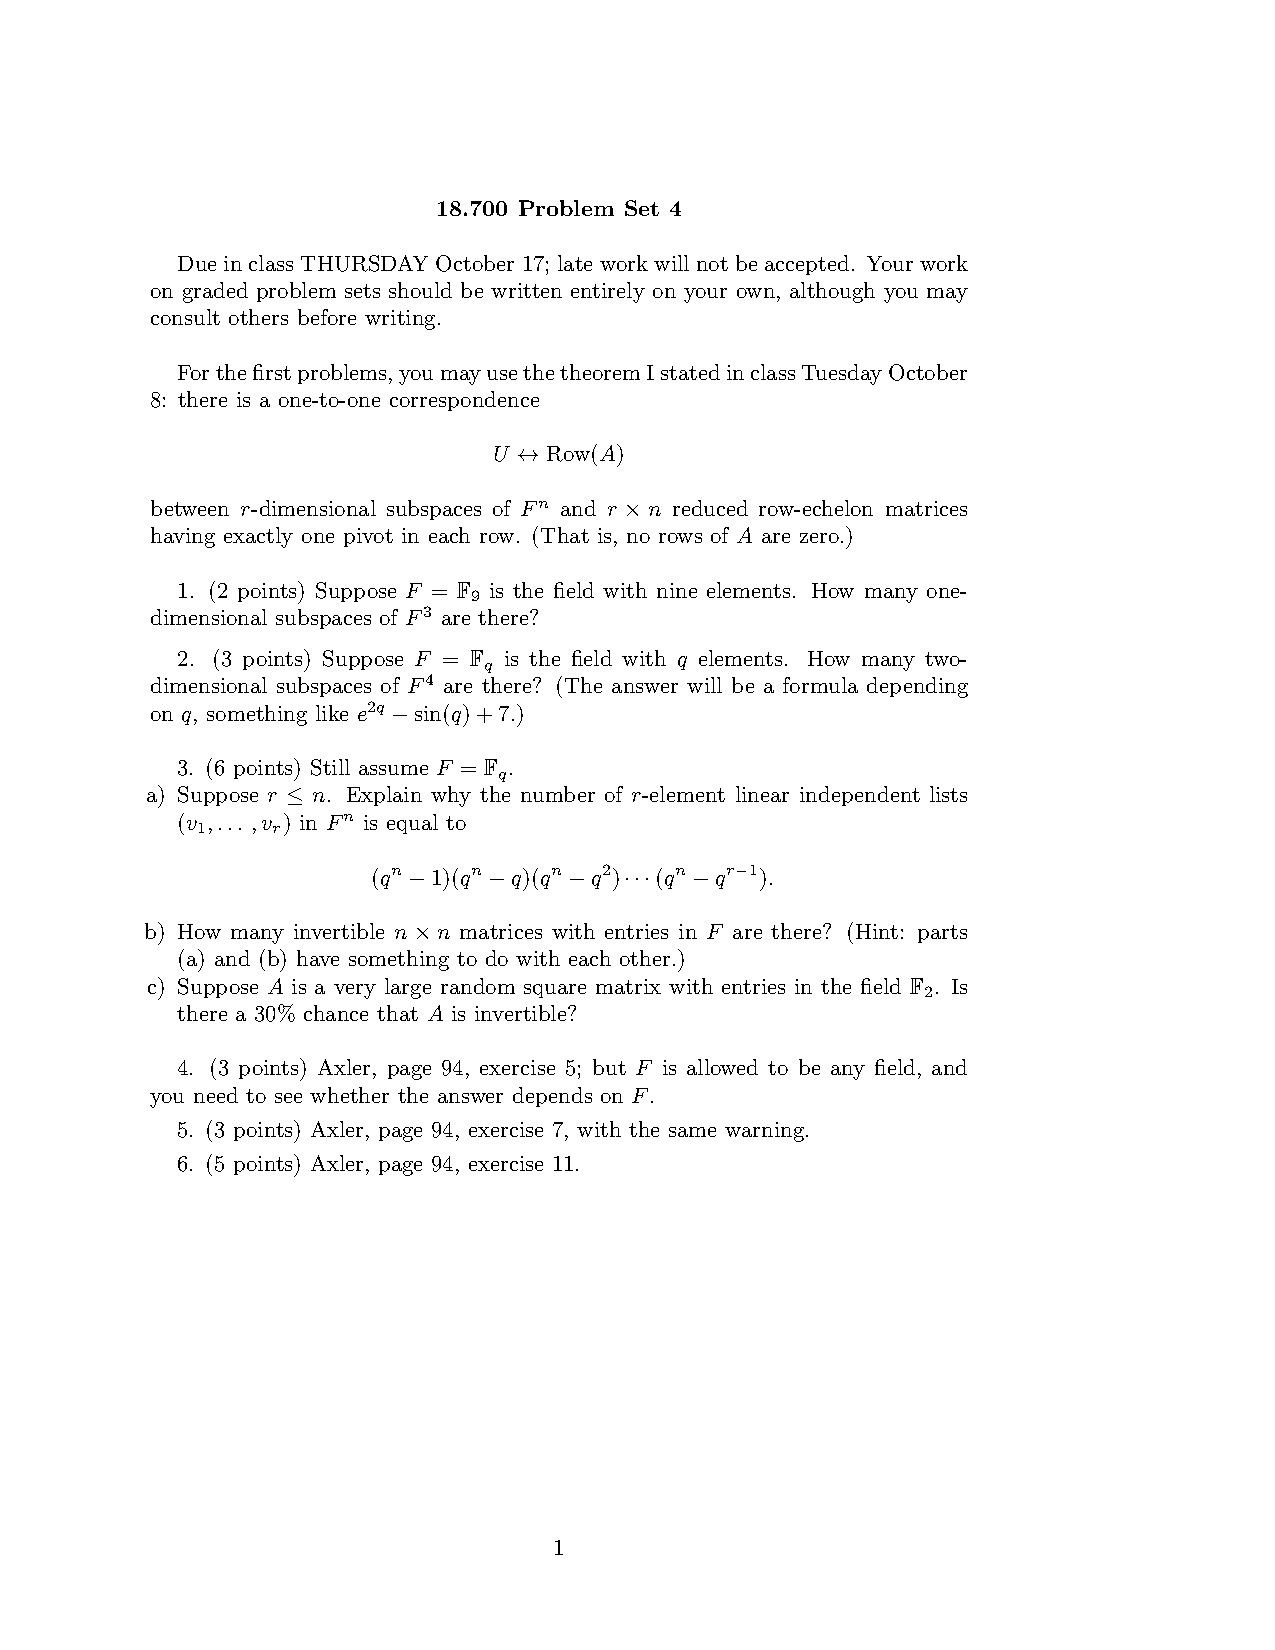
\includepdf[link=true, linkname=LinearAlgebra-ProblemSet4,pages=1]{MIT/Problems/18.700/ProblemSet4.pdf}
\section*{Question 1}
Since the subspaces are one to one mapped with the matrices in the row reduced echelon form, it is much easier to count those matrices.

The row reduced echelon form can be in one of the following 3 cases:

\begin{eqnarray*}
  \left(1, x, y\right)
  \left(0, 1, x\right)
  \left(0, 0, 1\right)
\end{eqnarray*}

There are $ 9 \times 9 = 81 $ different matrices of the first form. $ 9 $ matrices of the second form and 1 matrix of the last form. There are $ 81 + 9 + 1 = 91 $ different row educed echelon matrices, and therefore there are 91 different subspace of 1 dimension.

To verify this is the right solution, I started learning \href{https://www.sagemath.org/}{Sage}. Here is some sage code that verify that there is indeed 91 subspaces. The code simply iterate through all possible vectors in $ F^3 $ and then canonicalize them using the echelon form and count how many distinct subspaces there are. Obviously, we must discount the $ \left(0, 0, 0\right) $ special case for safety sake.

\begin{verbatim}
Field = GF(9)
MatrixOnField = MatrixSpace(Field,1,3)
elements = []
for _,element in enumerate(Field):
  elements.append(element)
Subspaces = {}
for p in elements:
  for q in elements:
    for r in elements:
      Reduced = MatrixOnField([p,q,r]).echelon_form()
      if Reduced[0] != MatrixOnField([0,0,0])[0]:
        Subspaces[Reduced] = True
len(Subspaces)
\end{verbatim}
\section*{Question 2}
Using the same idea as in question 1, the row reduced echelon form can be in one of the following cases:

\begin{eqnarray*}
  \left(
  \begin{array}{cccc}
  1, 0, a, b \\
  0, 1, c, d
  \end{array}
  \right) \\
  \left(
  \begin{array}{cccc}
  1, a, 0, b \\
  0, 0, 1, c
  \end{array}
  \right) \\
  \left(
  \begin{array}{cccc}
  1, a, b, 0 \\
  0, 0, 0, 1
  \end{array}
  \right) \\
  \left(
  \begin{array}{cccc}
  0, 1, 0, a \\
  0, 0, 1, b
  \end{array}
  \right) \\
  \left(
  \begin{array}{cccc}
  0, 1, a, 0 \\
  0, 0, 0, 1
  \end{array}
  \right) \\
  \left(
  \begin{array}{cccc}
  0, 0, 1, 0 \\
  0, 0, 0, 1
  \end{array}
  \right)
\end{eqnarray*}
Using these cases, we will have $ q^4 + q^3 + 2q^2 + q + 1 $ row reduced echelon matrices, and therefore having the same number of vector subspaces of dimension 2.
\section*{Question 3}
\subsection*{Part a}
In $ F^n $, there are $ q^n $ vectors. One of them is the zero vector that we must exclude. Otherwise, all $ q^n - 1 $ vector could be the first vector in the list. That's why we have the $ (q^n - 1) $ as the first factor.

For each vector $ v $ as the first vector, $ \{ v, 2v, \cdots (q-1)v \} $ is a set of $ q - 1 $ vectors that should also be excluded as the second vector. That gives us the second factor of $ (q^n - 1) - (q - 1) = (q^n - q) $.

For each pair of vector $ v $ and $ w $ as the first two vectors, $ \{ v, v + w, \cdots, v + (q-1)w, 2v, 2v + w, \cdots 2v + (q-1)w, \cdots (q-1)v + (q-1)w \} $ is a set of $ (q^2 - 1) $ vectors that should be excluded as the third vector. That gives us the third factor of $ (q^n - 1) - (q^2 - 1) = (q^n - q^2) $.

The argument goes on and eventually lead to the expression we wanted.

\subsection*{Part b}
An $ n \times n $ invertible matrix is simply a list of $ n $ linearly independent (column) vectors. So the number of invertible matrices is $ (q^n - 1)(q^n - q)\cdots(q^n - q^{n-1})$

\section*{Part c}
Suppose we already know $ (2^k - 1)(2^k - 2)\cdots(2^k - 2^{k-1}) $, to compute $ (2^{k+1} - 1)(2^{k+1} - 2)\cdots(2^{k+1} - 2^k) $ can be done by multiplying all the terms by $ q $ and multiply an extra term as follow:

\begin{eqnarray*}
  & & N_{k+1} \\
  &=& (2^{k+1} - 1)(2^{k+1} - 2) \cdots (2^{k+1} - 2^k) \\
  &=& (2^{k+1} - 1)2(2^k - 1) \cdots 2 (2^k - 2^{k-1}) \\
  &=& (2^{k+1} - 1)2^k N_k 
\end{eqnarray*}

$ N_k $ is the number of $ k \times k $ inverible matrices in $ F_2 $.

$ D_k $, the number of $ k \times k $  matrices in $ F_2 $ is simply $ 2^{k^2} $. We can also express it in an recurrence relation as follow:

\begin{eqnarray*}
  & & D_{k+1} \\
  &=& 2^{(k+1)^2} \\
  &=& 2^{k^2 + 2k + 1} \\
  &=& 2^{2k+1}D_k
\end{eqnarray*}

Now we can express $ P_k $, the probability that a $ k \times k $ random matrix in $ F_2 $ using the recurrence relation:

\begin{eqnarray*}
  & & P_{k+1} \\
  &=& \frac{N_{k+1}}{D_{k+1}} \\
  &=& \frac{(2^{k+1} - 1)2^k N_k }{2^{2k+1}D_k} \\
  &=& \frac{(2^{k+1} - 1)}{2^{k+1}}P_k \\
\end{eqnarray*}

That means the probabilities have a particular simple pattern of

\begin{eqnarray*}
  \frac{1}{2}, \frac{1}{2} \times \frac{3}{4}, \frac{1}{2} \times \frac{3}{4} \times \frac{7}{8}, \cdots
\end{eqnarray*}

This is obviously a strictly decreasing sequence and lower bounded by 0, it must have a limit. Numerically, the limiting value is $ 0.2887880952... $. That is very close to the given 30\% chance.

As an amusing fact, the number $ 0.2887880952 $ is found in the diehard random number testing suite. The test was trying to make sure if a random number generator is good, a random 32 x 32 matrix on $ F_2 $ should have this probability of being invertible. That means our calculations are good.
\section*{Question 4}
For any field $ F $, we have 1 and -1. (-1 is defined as the additive inverse of 1, which is usually not represented using the -1 symbol in finite fields).

Consider $ T(1,1) = (1,1) = 1(1,1) $ and $ T(1, -1) = (-1,1) = -1(1,-1) $. Therefore, 1 and -1 are the eigenvalues of $ T $.

Since $ T $ is a linear transformation from $ F^2 \to F^2 $, it has at most two eigenvalues, therefore $ \{1, -1\} $ are all the eigenvalues of $ T $.
\section*{Question 5}
Consider the vector of all 1.

\begin{eqnarray*}
T(1,1,\cdots,1) = (1+1+\cdots+1,1+1+\cdots+1,\cdots,1+1+\cdots+1) = (1+1+\cdots+1)(1,1,\cdots,1)
\end{eqnarray*}

It is cumbersome to write $ 1+1+\cdots+1 $ all the time, let's denote that as $ N $. In finite fields, that could be any element in the field, including $ 0 $. The above equation shows that $ N $ is an eigenvalue of $ T $.

Here is another way to construct and eigenvector:

\begin{eqnarray*}
T(1,0,0,\cdots,-1) = (0,0,\cdots,0) = 0(1,0,0,\cdots,-1)
\end{eqnarray*}

Again, -1 denotes the additive inverse of 1. The above equation shows that $ 0 $ is an eigenvalue of $ T $

The initial $ 1 $ can be placed anywhere in the first $ (n-1) $ dimensions as long as the last dimension is $ -1 $, this created $ (n-1) $ linearly independent vectors that spans the null space of $ T $.

Suppose $ N \ne 0 $, now we have two distinct eigenvalues, $ \{ N, 0 \} $, the eigenspace corresponding to $ N $ has dimension 1. The eigenspace corresponding to $ 0 $ has dimension $ n - 1 $. Therefore we have found all the eigenvalues.

On the other hand, if $ N = 0 $, we wanted to show that 0 is the only eigenvalue of $ T $. Consider a general case where we have $ T(x) = \lambda x $. In order for this to work, $ x $ must be a non-zero uniform vector, but then $ T(x) = 0 $, so $ \lambda $ must be 0.

As a side note, since $ dim(range(T)) = 1 $, $ dim(null(T)) = (n-1) $. When $ N = 0$, we know that $ \{0\} $ is the only eigenvalue, therefore the eigenspace corresponding to $ 0 $ is exactly the null space and has dimension $ (n - 1) $, that means the matrix is defective.
\section*{Question 6}
If $ \lambda $ is an eigenvalue of $ ST $, then there exists vector $ v $ such that $ ST(v) = \lambda v $.

Consider $ TS(T(v)) = T(ST(v)) = T(\lambda v) = \lambda T(v) $, this indicates $ \lambda $ is an eigenvalue of $ TS $.

Every eigenvalue of $ ST $ is an eigenvalue of $ TS $. Symmetrically, we can have every eigenvalue of $ TS $ is an eigenvalue of $ ST $. Therefore, these two linear transformations have exactly the same set of eigenvalues.

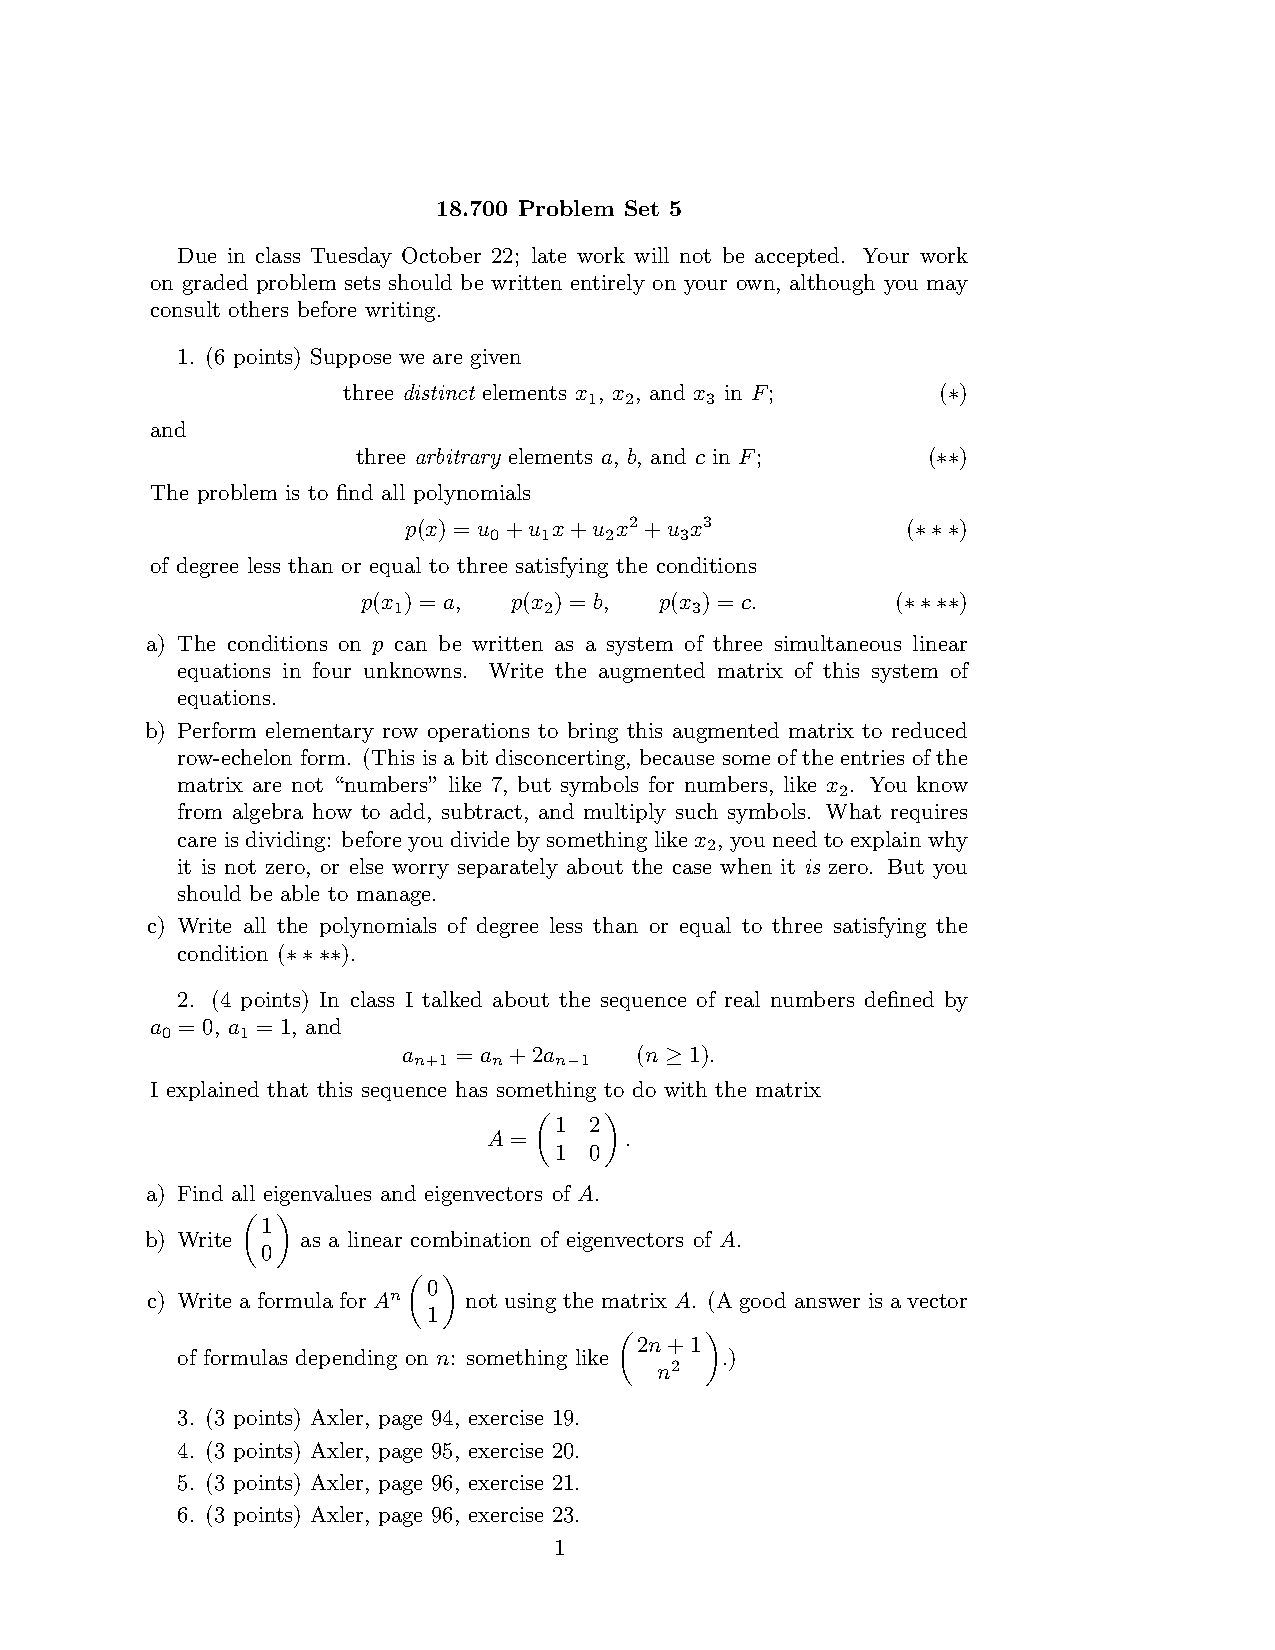
\includepdf[link=true, linkname=LinearAlgebra-ProblemSet5,pages=1]{MIT/Problems/18.700/ProblemSet5.pdf}
\section*{Question 1}
\subsection*{Part a}
\begin{eqnarray*}
\left(\begin{array}{rrrr|r}
1 & x_{1} & x_{1}^{2} & x_{1}^{3} & a \\
1 & x_{2} & x_{2}^{2} & x_{2}^{3} & b \\
1 & x_{3} & x_{3}^{2} & x_{3}^{3} & c
\end{array}\right)
\end{eqnarray*}
\subsection*{Part b}
Here we start:
\begin{eqnarray*}
\left(\begin{array}{rrrr|r}
1 & x_{1} & x_{1}^{2} & x_{1}^{3} & a \\
1 & x_{2} & x_{2}^{2} & x_{2}^{3} & b \\
1 & x_{3} & x_{3}^{2} & x_{3}^{3} & c
\end{array}\right)
\end{eqnarray*}
Subtract the second row by the first.
\begin{eqnarray*}
\left(\begin{array}{rrrr|r}
1 & x_{1} & x_{1}^{2} & x_{1}^{3} & a \\
0 & -x_{1} + x_{2} & -x_{1}^{2} + x_{2}^{2} & -x_{1}^{3} + x_{2}^{3} & -a + b \\
1 & x_{3} & x_{3}^{2} & x_{3}^{3} & c
\end{array}\right)
\end{eqnarray*}
We introduced some difference of powers, they can be factorized.
\begin{eqnarray*}
\left(\begin{array}{rrrr|r}
1 & x_{1} & x_{1}^{2} & x_{1}^{3} & a \\
0 & -x_{1} + x_{2} & -{\left(x_{1} + x_{2}\right)} {\left(x_{1} - x_{2}\right)} & -{\left(x_{1}^{2} + x_{1} x_{2} + x_{2}^{2}\right)} {\left(x_{1} - x_{2}\right)} & -a + b \\
1 & x_{3} & x_{3}^{2} & x_{3}^{3} & c
\end{array}\right)
\end{eqnarray*}
Subtract the third row by the first.
\begin{eqnarray*}
\left(\begin{array}{rrrr|r}
1 & x_{1} & x_{1}^{2} & x_{1}^{3} & a \\
0 & -x_{1} + x_{2} & -{\left(x_{1} + x_{2}\right)} {\left(x_{1} - x_{2}\right)} & -{\left(x_{1}^{2} + x_{1} x_{2} + x_{2}^{2}\right)} {\left(x_{1} - x_{2}\right)} & -a + b \\
0 & -x_{1} + x_{3} & -x_{1}^{2} + x_{3}^{2} & -x_{1}^{3} + x_{3}^{3} & -a + c
\end{array}\right)
\end{eqnarray*}
Again, we have some difference of powers, they can be factorized as well.
\begin{eqnarray*}
\left(\begin{array}{rrrr|r}
1 & x_{1} & x_{1}^{2} & x_{1}^{3} & a \\
0 & -x_{1} + x_{2} & -{\left(x_{1} + x_{2}\right)} {\left(x_{1} - x_{2}\right)} & -{\left(x_{1}^{2} + x_{1} x_{2} + x_{2}^{2}\right)} {\left(x_{1} - x_{2}\right)} & -a + b \\
0 & -x_{1} + x_{3} & -{\left(x_{1} + x_{3}\right)} {\left(x_{1} - x_{3}\right)} & -{\left(x_{1}^{2} + x_{1} x_{3} + x_{3}^{2}\right)} {\left(x_{1} - x_{3}\right)} & -a + c
\end{array}\right)
\end{eqnarray*}
With the factorization, we can easily scale down the second row.
\begin{eqnarray*}
\left(\begin{array}{rrrr|r}
1 & x_{1} & x_{1}^{2} & x_{1}^{3} & a \\
0 & 1 & x_{1} + x_{2} & x_{1}^{2} + x_{1} x_{2} + x_{2}^{2} & \frac{a - b}{x_{1} - x_{2}} \\
0 & -x_{1} + x_{3} & -{\left(x_{1} + x_{3}\right)} {\left(x_{1} - x_{3}\right)} & -{\left(x_{1}^{2} + x_{1} x_{3} + x_{3}^{2}\right)} {\left(x_{1} - x_{3}\right)} & -a + c
\end{array}\right)
\end{eqnarray*}
And scale down the third row as well
\begin{eqnarray*}
\left(\begin{array}{rrrr|r}
1 & x_{1} & x_{1}^{2} & x_{1}^{3} & a \\
0 & 1 & x_{1} + x_{2} & x_{1}^{2} + x_{1} x_{2} + x_{2}^{2} & \frac{a - b}{x_{1} - x_{2}} \\
0 & 1 & x_{1} + x_{3} & x_{1}^{2} + x_{1} x_{3} + x_{3}^{2} & \frac{a - c}{x_{1} - x_{3}}
\end{array}\right)
\end{eqnarray*}
Subtract the first row by the second row multiplied by $ x_1 $ times.
\begin{eqnarray*}
\left(\begin{array}{rrrr|r}
1 & 0 & -{\left(x_{1} + x_{2}\right)} x_{1} + x_{1}^{2} & x_{1}^{3} - {\left(x_{1}^{2} + x_{1} x_{2} + x_{2}^{2}\right)} x_{1} & a - \frac{{\left(a - b\right)} x_{1}}{x_{1} - x_{2}} \\
0 & 1 & x_{1} + x_{2} & x_{1}^{2} + x_{1} x_{2} + x_{2}^{2} & \frac{a - b}{x_{1} - x_{2}} \\
0 & 1 & x_{1} + x_{3} & x_{1}^{2} + x_{1} x_{3} + x_{3}^{2} & \frac{a - c}{x_{1} - x_{3}}
\end{array}\right)
\end{eqnarray*}
Note that we could cancel some terms if we expand it.
\begin{eqnarray*}
\left(\begin{array}{rrrr|r}
1 & 0 & -x_{1} x_{2} & -x_{1}^{2} x_{2} - x_{1} x_{2}^{2} & a - \frac{{\left(a - b\right)} x_{1}}{x_{1} - x_{2}} \\
0 & 1 & x_{1} + x_{2} & x_{1}^{2} + x_{1} x_{2} + x_{2}^{2} & \frac{a - b}{x_{1} - x_{2}} \\
0 & 1 & x_{1} + x_{3} & x_{1}^{2} + x_{1} x_{3} + x_{3}^{2} & \frac{a - c}{x_{1} - x_{3}}
\end{array}\right)
\end{eqnarray*}
Subtract the third row by the second row.
\begin{eqnarray*}
\left(\begin{array}{rrrr|r}
1 & 0 & -x_{1} x_{2} & -x_{1}^{2} x_{2} - x_{1} x_{2}^{2} & \frac{b x_{1} - a x_{2}}{x_{1} - x_{2}} \\
0 & 1 & x_{1} + x_{2} & x_{1}^{2} + x_{1} x_{2} + x_{2}^{2} & \frac{a - b}{x_{1} - x_{2}} \\
0 & 0 & -x_{2} + x_{3} & -x_{1} x_{2} - x_{2}^{2} + x_{1} x_{3} + x_{3}^{2} & \frac{b x_{1} - c x_{1} - a x_{2} + c x_{2} + a x_{3} - b x_{3}}{{\left(x_{1} - x_{2}\right)} {\left(x_{1} - x_{3}\right)}}
\end{array}\right)
\end{eqnarray*}
While it is not very clear, we can actually factorize the row 3 
\begin{eqnarray*}
\left(\begin{array}{rrrr|r}
1 & 0 & -x_{1} x_{2} & -x_{1}^{2} x_{2} - x_{1} x_{2}^{2} & \frac{b x_{1} - a x_{2}}{x_{1} - x_{2}} \\
0 & 1 & x_{1} + x_{2} & x_{1}^{2} + x_{1} x_{2} + x_{2}^{2} & \frac{a - b}{x_{1} - x_{2}} \\
0 & 0 & -x_{2} + x_{3} & -{\left(x_{1} + x_{2} + x_{3}\right)} {\left(x_{2} - x_{3}\right)} & \frac{b x_{1} - c x_{1} - a x_{2} + c x_{2} + a x_{3} - b x_{3}}{{\left(x_{1} - x_{2}\right)} {\left(x_{1} - x_{3}\right)}}
\end{array}\right)
\end{eqnarray*}
Now we can easily scale down row 3 after the factorization
\begin{eqnarray*}
\left(\begin{array}{rrrr|r}
1 & 0 & -x_{1} x_{2} & -x_{1}^{2} x_{2} - x_{1} x_{2}^{2} & \frac{b x_{1} - a x_{2}}{x_{1} - x_{2}} \\
0 & 1 & x_{1} + x_{2} & x_{1}^{2} + x_{1} x_{2} + x_{2}^{2} & \frac{a - b}{x_{1} - x_{2}} \\
0 & 0 & 1 & x_{1} + x_{2} + x_{3} & -\frac{b x_{1} - c x_{1} - a x_{2} + c x_{2} + a x_{3} - b x_{3}}{{\left(x_{1} - x_{2}\right)} {\left(x_{1} - x_{3}\right)} {\left(x_{2} - x_{3}\right)}}
\end{array}\right)
\end{eqnarray*}
Subtract the second row by the third row multiplied by $ x_1 + x_2 $ times.
\begin{eqnarray*}
\left(\begin{array}{rrrr|r}
1 & 0 & -x_{1} x_{2} & -x_{1}^{2} x_{2} - x_{1} x_{2}^{2} & \frac{b x_{1} - a x_{2}}{x_{1} - x_{2}} \\
0 & 1 & 0 & -{\left(x_{1} + x_{2} + x_{3}\right)} {\left(x_{1} + x_{2}\right)} + x_{1}^{2} + x_{1} x_{2} + x_{2}^{2} & \frac{b x_{1}^{2} - c x_{1}^{2} - a x_{2}^{2} + c x_{2}^{2} + a x_{3}^{2} - b x_{3}^{2}}{{\left(x_{1} - x_{2}\right)} {\left(x_{1} - x_{3}\right)} {\left(x_{2} - x_{3}\right)}} \\
0 & 0 & 1 & x_{1} + x_{2} + x_{3} & -\frac{b x_{1} - c x_{1} - a x_{2} + c x_{2} + a x_{3} - b x_{3}}{{\left(x_{1} - x_{2}\right)} {\left(x_{1} - x_{3}\right)} {\left(x_{2} - x_{3}\right)}}
\end{array}\right)
\end{eqnarray*}
Observe that some terms cancel if we expand the product
\begin{eqnarray*}
\left(\begin{array}{rrrr|r}
1 & 0 & -x_{1} x_{2} & -x_{1}^{2} x_{2} - x_{1} x_{2}^{2} & \frac{b x_{1} - a x_{2}}{x_{1} - x_{2}} \\
0 & 1 & 0 & -x_{1} x_{2} - x_{1} x_{3} - x_{2} x_{3} & \frac{b x_{1}^{2} - c x_{1}^{2} - a x_{2}^{2} + c x_{2}^{2} + a x_{3}^{2} - b x_{3}^{2}}{{\left(x_{1} - x_{2}\right)} {\left(x_{1} - x_{3}\right)} {\left(x_{2} - x_{3}\right)}} \\
0 & 0 & 1 & x_{1} + x_{2} + x_{3} & -\frac{b x_{1} - c x_{1} - a x_{2} + c x_{2} + a x_{3} - b x_{3}}{{\left(x_{1} - x_{2}\right)} {\left(x_{1} - x_{3}\right)} {\left(x_{2} - x_{3}\right)}}
\end{array}\right)
\end{eqnarray*}
Add the first row by the third row multiplied by $ x_1 x_2 $ times.
\begin{eqnarray*}
\left(\begin{array}{rrrr|r}
1 & 0 & 0 & {\left(x_{1} + x_{2} + x_{3}\right)} x_{1} x_{2} - x_{1}^{2} x_{2} - x_{1} x_{2}^{2} & \frac{c x_{1}^{2} x_{2} - c x_{1} x_{2}^{2} - b x_{1}^{2} x_{3} + a x_{2}^{2} x_{3} + b x_{1} x_{3}^{2} - a x_{2} x_{3}^{2}}{{\left(x_{1} - x_{2}\right)} {\left(x_{1} - x_{3}\right)} {\left(x_{2} - x_{3}\right)}} \\
0 & 1 & 0 & -x_{1} x_{2} - x_{1} x_{3} - x_{2} x_{3} & \frac{b x_{1}^{2} - c x_{1}^{2} - a x_{2}^{2} + c x_{2}^{2} + a x_{3}^{2} - b x_{3}^{2}}{{\left(x_{1} - x_{2}\right)} {\left(x_{1} - x_{3}\right)} {\left(x_{2} - x_{3}\right)}} \\
0 & 0 & 1 & x_{1} + x_{2} + x_{3} & -\frac{b x_{1} - c x_{1} - a x_{2} + c x_{2} + a x_{3} - b x_{3}}{{\left(x_{1} - x_{2}\right)} {\left(x_{1} - x_{3}\right)} {\left(x_{2} - x_{3}\right)}}
\end{array}\right)
\end{eqnarray*}
Again, observe that some terms cancel if we expand the product
\begin{eqnarray*}
\left(\begin{array}{rrrr|r}
1 & 0 & 0 & x_{1} x_{2} x_{3} & \frac{c x_{1}^{2} x_{2} - c x_{1} x_{2}^{2} - b x_{1}^{2} x_{3} + a x_{2}^{2} x_{3} + b x_{1} x_{3}^{2} - a x_{2} x_{3}^{2}}{{\left(x_{1} - x_{2}\right)} {\left(x_{1} - x_{3}\right)} {\left(x_{2} - x_{3}\right)}} \\
0 & 1 & 0 & -x_{1} x_{2} - x_{1} x_{3} - x_{2} x_{3} & \frac{b x_{1}^{2} - c x_{1}^{2} - a x_{2}^{2} + c x_{2}^{2} + a x_{3}^{2} - b x_{3}^{2}}{{\left(x_{1} - x_{2}\right)} {\left(x_{1} - x_{3}\right)} {\left(x_{2} - x_{3}\right)}} \\
0 & 0 & 1 & x_{1} + x_{2} + x_{3} & -\frac{b x_{1} - c x_{1} - a x_{2} + c x_{2} + a x_{3} - b x_{3}}{{\left(x_{1} - x_{2}\right)} {\left(x_{1} - x_{3}\right)} {\left(x_{2} - x_{3}\right)}}
\end{array}\right)
\end{eqnarray*}
Observe that we have a very nice symmetric left hand side while the right hand side is a mess. The issue is that $ a, b, c $ make the problem asymmetric, and they are all concentrated at the last column, that is why that column looks particular complicated.

Doing these tedious manipulation is very error prone, and therefore it is best left for the computer. Sage is capable to produce a reduced echelon form directly, but it make questionable division and produced a matrix that is very complicated. In order to reach this relatively simple form, I need to guide it to do the right simplification at the right time. For the record, here is the code used to produce the \LaTeX above. 
\begin{verbatim}
%typeset_mode True

p = var("x_1")
q = var("x_2")
r = var("x_3")
a = var("a")
b = var("b")
c = var("c")
l1 = Matrix([[1,p,p^2,p^3],[1,q,q^2,q^3],[1,r,r^2,r^3]])
r1 = Matrix([[a],[b],[c]])

print("Here we start:")
print("\\begin{eqnarray*}")
latex(l1.augment(r1))
print("\\end{eqnarray*}")

l2 = l1.with_added_multiple_of_row(1,0,-1)
r2 = r1.with_added_multiple_of_row(1,0,-1).factor().simplify()

print("Subtract the second row by the first.")
print("\\begin{eqnarray*}")
latex(l2.augment(r2))
print("\\end{eqnarray*}")

l3 = l2
r3 = r2
l3[1,2] = l3[1,2].factor()
l3[1,3] = l3[1,3].factor()

print("We introduced some difference of powers, they can be factorized.")
print("\\begin{eqnarray*}")
latex(l3.augment(r3))
print("\\end{eqnarray*}")

l4 = l3.with_added_multiple_of_row(2,0,-1)
r4 = r3.with_added_multiple_of_row(2,0,-1).factor().simplify()

print("Subtract the third row by the first.")
print("\\begin{eqnarray*}")
latex(l4.augment(r4))
print("\\end{eqnarray*}")

l5 = l4
r5 = r4
l5[2,2] = l5[2,2].factor()
l5[2,3] = l5[2,3].factor()

print("Again, we have some difference of powers, they can be factorized as well.")
print("\\begin{eqnarray*}")
latex(l5.augment(r5))
print("\\end{eqnarray*}")

l6 = l5.with_rescaled_row(1,1/(q-p))
r6 = r5.with_rescaled_row(1,1/(q-p)).factor().simplify()

print("With the factorization, we can easily scale down the second row.")
print("\\begin{eqnarray*}")
latex(l6.augment(r6))
print("\\end{eqnarray*}")

l7 = l6.with_rescaled_row(2,1/(r-p))
r7 = r6.with_rescaled_row(2,1/(r-p)).factor().simplify()

print("And scale down the third row as well")
print("\\begin{eqnarray*}")
latex(l7.augment(r7))
print("\\end{eqnarray*}")

l8 = l7.with_added_multiple_of_row(0,1,-p)
r8 = r7.with_added_multiple_of_row(0,1,-p)

print("Subtract the first row by the second row multiplied by $ x_1 $ times.")
print("\\begin{eqnarray*}")
latex(l8.augment(r8))
print("\\end{eqnarray*}")

l9 = l8
r9 = r8
l9[0,2] = l9[0,2].expand().simplify()
l9[0,3] = l9[0,3].expand().simplify()

print("Note that we could cancel some terms if we expand it.")
print("\\begin{eqnarray*}")
latex(l9.augment(r9))
print("\\end{eqnarray*}")

l10 = l9.with_added_multiple_of_row(2,1,-1)
r10 = r9.with_added_multiple_of_row(2,1,-1).factor().simplify()

print("Subtract the third row by the second row.")
print("\\begin{eqnarray*}")
latex(l10.augment(r10))
print("\\end{eqnarray*}")

l11 = l10
r11 = r10
l11[2,3] = l11[2,3].factor()

print("While it is not very clear, we can actually factorize the row 3 ")
print("\\begin{eqnarray*}")
latex(l11.augment(r11))
print("\\end{eqnarray*}")

l12 = l11.with_rescaled_row(2,1/(r-q))
r12 = r11.with_rescaled_row(2,1/(r-q)).factor().simplify()

print("Now we can easily scale down row 3 after the factorization")
print("\\begin{eqnarray*}")
latex(l12.augment(r12))
print("\\end{eqnarray*}")

l13 = l12.with_added_multiple_of_row(1,2,-p-q)
r13 = r12.with_added_multiple_of_row(1,2,-p-q).factor().simplify()

print("Subtract the second row by the third row multiplied by $ x_1 + x_2 $ times.")
print("\\begin{eqnarray*}")
latex(l13.augment(r13))
print("\\end{eqnarray*}")

l14 = l13
r14 = r13
l14[1,3] = l14[1,3].expand().simplify()

print("Observe that some terms cancel if we expand the product")
print("\\begin{eqnarray*}")
latex(l14.augment(r14))
print("\\end{eqnarray*}")

l15 = l14.with_added_multiple_of_row(0,2,p*q)
r15 = r14.with_added_multiple_of_row(0,2,p*q).factor().simplify()

print("Add the first row by the third row multiplied by $ x_1 x_2 $ times.")
print("\\begin{eqnarray*}")
latex(l15.augment(r15))
print("\\end{eqnarray*}")

l16 = l15
r16 = r15
l16[0,3] = l16[0,3].expand().simplify()

print("Again, observe that some terms cancel if we expand the product")
print("\\begin{eqnarray*}")
latex(l16.augment(r16))
print("\\end{eqnarray*}")
\end{verbatim}
Even with computer, this is taking me a lot of hours, and this is a bad approach to solve this problem, as we will see in the next part.
\subsection*{Part c}
We can easily find a polynomial satisfying the constraint using Lagrange's interpolation as follow:
\begin{eqnarray*}
    \frac{(x - x_2)(x - x_3)}{(x_1 - x_2)(x_1 - x_3)} a + \frac{(x - x_1)(x - x_3)}{(x_2 - x_1)(x_2 - x_3)} b + \frac{(x - x_1)(x - x_2)}{(x_3 - x_1)(x_3 - x_2)} c
\end{eqnarray*}
Now suppose we have two such polynomials $ f $ and $ g $. we notice that $ f - g $ must have three roots at $ \{ x_1, x_2, x_3\} $, that means $ f - g = n(x - x_1)(x-x_2)(x - x_3) $ for an arbitrary $ n \in F $.

So the solution is simply 
\begin{eqnarray*}
    \frac{(x - x_2)(x - x_3)}{(x_1 - x_2)(x_1 - x_3)} a + \frac{(x - x_1)(x - x_3)}{(x_2 - x_1)(x_2 - x_3)} b + \frac{(x - x_1)(x - x_2)}{(x_3 - x_1)(x_3 - x_2)} c + n(x - x_1)(x-x_2)(x - x_3)
\end{eqnarray*}

Note how this solution ressemble the reduced echelon form we found in part b. The denominator on the right hand side comes from the Lagrange interpolation, and the symmetric polynomials on the left hand side comes from the expansion of  $ (x - x_1)(x-x_2)(x - x_3) $. This also shows the solution lies in a one dimensional subspace of $ F_4 $, which also agree with the reduced echelon form.
\section*{Question 2}
\subsection*{Part a}
\begin{eqnarray*}
\left(\begin{array}{cc}
1 & 2 \\
1 & 0
\end{array}\right)
\left(\begin{array}{c}
x \\
y
\end{array}\right) &=&
\lambda
\left(\begin{array}{c}
x \\
y
\end{array}\right) \\
\left(\begin{array}{cc}
1 & 2 \\
1 & 0
\end{array}\right)
\left(\begin{array}{c}
x \\
y
\end{array}\right) -
\lambda
\left(\begin{array}{c}
x \\
y
\end{array}\right) &=& 0 \\
\left[
\left(\begin{array}{cc}
1 & 2 \\
1 & 0
\end{array}\right)
- \lambda I
\right]
\left(\begin{array}{c}
x \\
y
\end{array}\right) &=& 0 \\
\det\left[
\left(\begin{array}{cc}
1 & 2 \\
1 & 0
\end{array}\right)
- \lambda I
\right] &=& 0 \\
(1 - \lambda)(-\lambda) - 2 &=& 0 \\
\lambda^2 - \lambda - 2 &=& 0 \\
(\lambda + 1)(\lambda - 2) &=& 0  
\end{eqnarray*}
When $ \lambda = -1 $, we have
\begin{eqnarray*}
\left(\begin{array}{cc}
1 & 2 \\
1 & 0
\end{array}\right)
\left(\begin{array}{c}
x \\
y
\end{array}\right) &=&
-
\left(\begin{array}{c}
x \\
y
\end{array}\right) \\
\left(\begin{array}{c}
x + 2y \\
x
\end{array}\right) &=&
-
\left(\begin{array}{c}
x \\
y
\end{array}\right) \\
\end{eqnarray*}
So we find $ (1, -1)^T $ is an eigenvector corresponding to the eigenvalue -1.

When $ \lambda = 2 $, we have
\begin{eqnarray*}
\left(\begin{array}{cc}
1 & 2 \\
1 & 0
\end{array}\right)
\left(\begin{array}{c}
x \\
y
\end{array}\right) &=&
2
\left(\begin{array}{c}
x \\
y
\end{array}\right) \\
\left(\begin{array}{c}
x + 2y \\
x
\end{array}\right) &=&
\left(\begin{array}{c}
2x \\
2y
\end{array}\right) \\
\end{eqnarray*}
So we find $ (2, 1)^T $ is an eigenvector corresponding to the eigenvalue 2.
\subsection*{Part b}
By inspection:
\begin{eqnarray*}
\left(\begin{array}{c}
3 \\
0
\end{array}\right) &=& 
\left(\begin{array}{c}
2 \\
1
\end{array}\right)
+
\left(\begin{array}{c}
1 \\
-1
\end{array}\right) \\
\left(\begin{array}{c}
1 \\
0
\end{array}\right) &=& 
\frac{1}{3}\left(\begin{array}{c}
2 \\
1
\end{array}\right)
+
\frac{1}{3}\left(\begin{array}{c}
1 \\
-1
\end{array}\right)
\end{eqnarray*}
\subsection*{Part c}
Like part b, we can also have:
\begin{eqnarray*}
\left(\begin{array}{c}
0 \\
3
\end{array}\right) &=& 
\left(\begin{array}{c}
2 \\
1
\end{array}\right)
-2
\left(\begin{array}{c}
1 \\
-1
\end{array}\right) \\
\left(\begin{array}{c}
0 \\
1
\end{array}\right) &=& 
\frac{1}{3}\left(\begin{array}{c}
2 \\
1
\end{array}\right)
-
\frac{2}{3}\left(\begin{array}{c}
1 \\
-1
\end{array}\right)
\end{eqnarray*}
Now we can solve
\begin{eqnarray*}
  & & A^n\left(\begin{array}{c}
0 \\
1
\end{array}\right) \\
  &=& A^n \left[\frac{1}{3}\left(\begin{array}{c}
2 \\
1
\end{array}\right)
-
\frac{2}{3}\left(\begin{array}{c}
1 \\
-1
\end{array}\right)\right] \\
  &=& \frac{1}{3}A^n\left(\begin{array}{c}
2 \\
1
\end{array}\right)
-
\frac{2}{3}A^n\left(\begin{array}{c}
1 \\
-1
\end{array}\right) \\
  &=& \frac{1}{3}2^n\left(\begin{array}{c}
2 \\
1
\end{array}\right)
-
\frac{2}{3}(-1)^n\left(\begin{array}{c}
1 \\
-1
\end{array}\right) \\
  &=& \frac{1}{3}\left(\begin{array}{c}
2^{n+1} + 2(-1)^{n+1} \\
2^n + 2(-1)^n
\end{array}\right) \\
\end{eqnarray*}
\section*{Question 3}
The idea is to construct a matrix that has determinant 0. For convenience, let's try to construct a 2 x 2 example. The simplest non-zero diagonal is simply this:

\begin{eqnarray*}
\left(\begin{array}{cc}
1 & * \\
* & 1
\end{array}\right)
\end{eqnarray*}

Now it is easy to see that we want the two unknown to have product 1, and that can be easily achieved with 

\begin{eqnarray*}
\left(\begin{array}{cc}
1 & 1 \\
1 & 1
\end{array}\right)
\end{eqnarray*}

This can be interpreted as a linear transformation that takes $ av_1 + bv_2 $ to $ (a+b)v_1 + (a+b)v_2 $, and it is obviously non-invertible because it is not injective that both $ v_1 $ and $ v_2 $ maps to $ v_1 + v_2 $.
\section*{Question 4}
Since we have $ dim(V) $ distinct eigenvalues, the eigenvectors $ v_1, v_2 \cdots v_n $ form a basis, any vectors and be written as a linear combination of them. Denote the eigenvalues of $ v_i $ corresponding to $ S $ to be $ \lambda_{si} $ and corresponding to $ T $ to be $ \lambda_{ti} $.

Consider both $ ST $ applied to an arbitrary vector $ v $ as follow:

\begin{eqnarray*}
  & & ST v \\
  &=& ST (\sum c_i v_i) \\
  &=& \sum c_i ST v_i \\
  &=& \sum c_i S \lambda_{ti}v_i \\
  &=& \sum c_i \lambda_{ti} S v_i \\
  &=& \sum c_i \lambda_{ti} \lambda_{si} v_i \\
\end{eqnarray*}

Similarly, when applied to $ TS $, we have:

\begin{eqnarray*}
  & & TS v \\
  &=& TS (\sum c_i v_i) \\
  &=& \sum c_i TS v_i \\
  &=& \sum c_i T \lambda_{si}v_i \\
  &=& \sum c_i \lambda_{si} T v_i \\
  &=& \sum c_i \lambda_{si} \lambda_{ti} v_i \\
  &=& \sum c_i \lambda_{ti} \lambda_{si} v_i \\
  & & ST v \\
\end{eqnarray*}

Since the two linear transformation behave exactly the same to all vectors in $ V $, these two linear transformation are identical.
\section*{Question 5}
For every vector $ v $ in $ V $, we can decompose it as follow:

\begin{eqnarray*}
  v &=& Pv + (v - Pv)
\end{eqnarray*}

It is obvious that $ Pv \in range(P) $, now we show that $ v - Pv \in null(P) $ by checking:

\begin{eqnarray*}
  & & P(v - Pv) \\ 
  &=& Pv - P^2v \\
  &=& Pv - Pv \\
  &=& 0 
\end{eqnarray*}

Suppose there exists a vector $ s $ such that $ s \in range(P) \cap null(P) $, we have $ Pt = s $ and so:

\begin{eqnarray*}
     Ps &=& 0 \\
  P(Pt) &=& 0 \\
     Pt &=& 0 \\
      s &=& 0
\end{eqnarray*}

Therefore, $ range(P) \cap null(T) = \{0\} $ and so $ V = range(P) \bigoplus null(P) $.
\section*{Question 6}
We already knew that the rotate by 90 degree transformation in 2D does not have a real eigenvalue, can we do that same in $ R_4 $?

Why not? We can have this linear transformation $ T(a,b,c,d) = (-b,a,-d,c) $.

Here are the eigenvalues and eigenvectors in $ C $:

\begin{eqnarray*}
  T(1,i,0,0) &=& (-i,1,0,0)  \\
             &=& -i(1,i,0,0) \\
  T(i,1,0,0) &=& (-1,i,0,0)  \\
             &=& i(i,1,0,0)  \\
  T(0,0,1,i) &=& (0,0,-i,1,) \\
             &=& -i(0,0,1,i) \\
  T(0,0,i,1) &=& (0,0,-1,i)  \\
             &=& i(0,0,i,1)
\end{eqnarray*}

Note that these eigenvectors are linearly independent, therefore $ i $ and $ -i $ are the only eigenvalues in $ C $, that means it doesn't have an eigenvalue in $ R $.

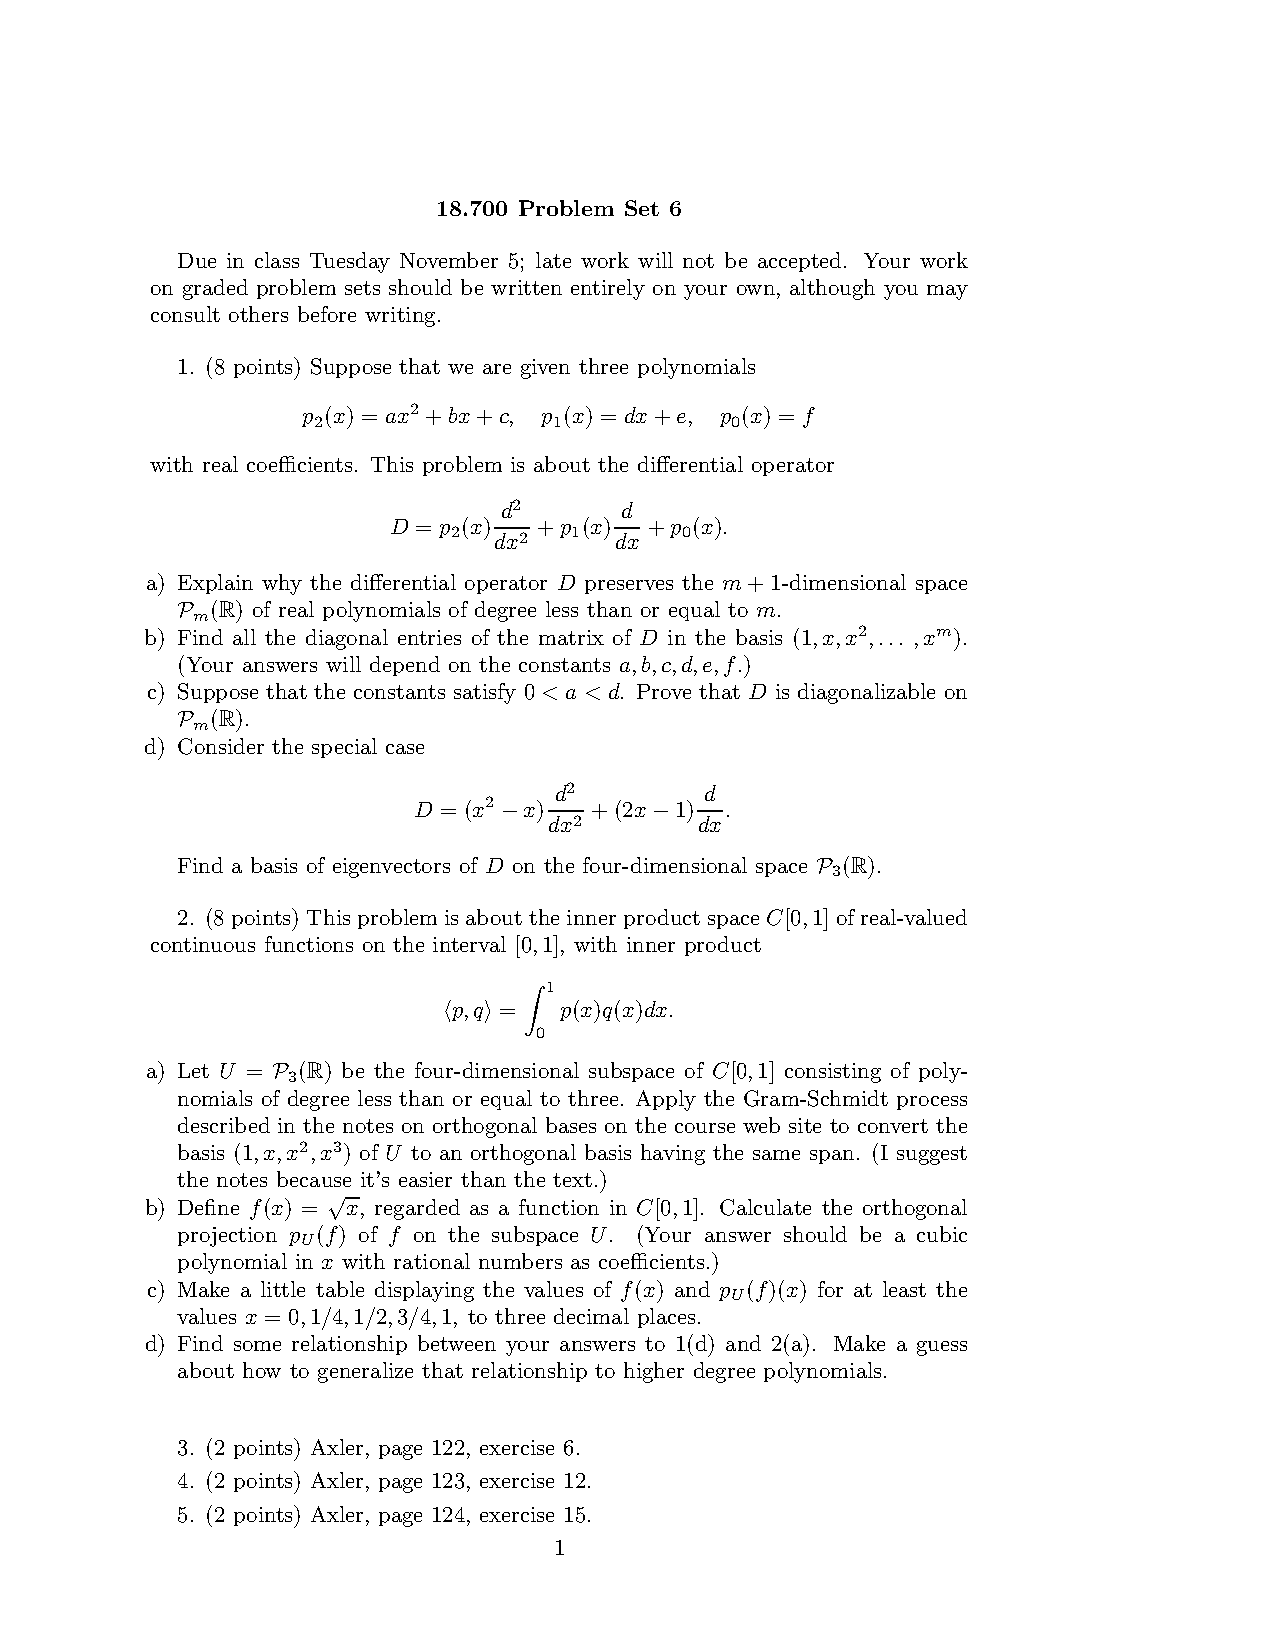
\includepdf[link=true, linkname=LinearAlgebra-ProblemSet6,pages=1]{MIT/Problems/18.700/ProblemSet6.pdf}
\section*{Question 1}
\subsection*{Part a}
It is unclear what "preserve" means in this context, but I can prove that the range is a subset of $ P_m(R) $. 

\begin{eqnarray*}
  & & deg(D p) \\
  &=& deg(p_2 \frac{d}{dx^2}p + p_1 \frac{d}{dx}p + p_0 p ) \\
  &\le& max(deg(p_2 \frac{d^2p}{dx^2}, deg(p_1 \frac{dp}{dx}), deg(p_0 p )) \\
  &\le& max(deg(p_2)+deg(\frac{d^2p}{dx^2}), deg(p_1)+deg(\frac{dp}{dx}), deg(p_0)deg(p)) \\
  &\le& max(2+(m-2), 1+(m-1), 0 + m) \\
  &=& m  
\end{eqnarray*}

Therefore the range of $ D $ is a subset of $ P_m(R) $.

\subsection*{Part b}
Consider $ D(x^k) $, we have these special cases:

\begin{eqnarray*}
  D x^0 &=& f \\
  D x^1 &=& dx + (e + f) \\
\end{eqnarray*}

For $ k \ge 2 $, we have

\begin{eqnarray*}
  & & D(x^k) \\
  &=& (ax^2 + bx + c)\frac{d^2}{dx}x^k + (dx + e)\frac{d}{dx}x^k + fx^k \\
  &=& (ax^2 + bx + c)k(k-1)x^{k-2} + (dx + e)kx^{k-1} + fx^k \\
  &=& k(k-1)(ax^k + bx^{k-1} + cx^{k-2}) + k(dx^k + ex^{k-1}) + fx^k \\
\end{eqnarray*}

The diagonal entries of the matrix correspond to the coefficient of $ x_k $. The first two are $ f $ and $ d $, the remaining ones are $ k(k-1)a + kd +f $ for $ k \ge 2 $.
\subsection*{Part c}
Suppose $ 0 < a < d $, 

\subsection*{Part d}
In case $ a = 1. b = -1, c = 0, d = 2, e = -1, f = 0 $, we have the polynomials:

\begin{eqnarray*}
  D(x^0) &=& 0 \\
  D(x^1) &=& 2x - 1 \\
  D(x^2) &=& 2(2-1)(x^2 - x^1) + 2(2x^2 - x^1) \\
         &=& 6x^2 - 4x \\
  D(x^3) &=& 3(3-1)(x^3 - x^2) + 3(2x^3 - x^2) \\
        &=& 12x^3 - 9x^2 \\
\end{eqnarray*}

The correspond to the matrix:
\begin{eqnarray*}
  & & M(D) \\
  &=& \left(\begin{array}{cccc}
    0 & -1 &  0 & 0  \\
    0 & 2  & -4 & 0  \\
    0 & 0  &  6 & -9 \\
    0 & 0  &  0 & 12
      \end{array}\right)
\end{eqnarray*}

The eigenvalues are obviously the ones on the diagonal, finding the eigenvectors is just a tedious exercise that is best done by the computer, here are the eigenvectors:

\begin{eqnarray*}
  D(1) &=& 0 \times 1 \\
  D(2x - 1) &=& 2 \times (2x - 1) \\
  D(6x^2 - 6x + 1) &=& 6 \times (6x^2 - 6x + 1) \\
  D(20x^3 - 30x^2 + 12x - 1) &=& 12 \times (20x^3 - 30x^2 + 12x - 1)
\end{eqnarray*}
\section*{Question 2}
\subsection*{Part a}
\begin{itemize}
    \item The first basis direction is $ d_1 = 1 $.
    \item The first basis vector is $ v_1 = \frac{d_1}{\sqrt{<d_1, d_1>}} = 1 $
    \item The second basis direction is $ d_2 = x - <x, v_1> v_1 = x - \frac{1}{2} $
    \item The second basis vector is $ \frac{d_2}{\sqrt{<d_2, d_2>}} = \sqrt{3}(2x - 1) $
    \item The third basis direction is $ d_3 = x^2 - <x^2, v_2> v_2 - <x^2, v_1> v_1 = x - \frac{1}{2} = x^2 - x + \frac{1}{6} $
    \item The third basis vector is $ v_3 = \frac{d_3}{\sqrt{<d_3, d_3>}} = \sqrt{5}(6x^2 - 6x + 1) $
    \item The fourth basis direction is $ d_4 = x^3 - <x^3, v_3> v_3 - <x^3, v_2> v_2  - <x^3, v_1> v_1 = \frac{1}{20}(20x^3 - 30x^2 + 12x - 1) $
    \item The fourth basis vector is $ v_4 = \frac{d_4}{\sqrt{<d_4, d_4>}} = \sqrt{7}(20x^3 - 30x^2 + 12x - 1) $
\end{itemize}
\subsection*{Part b}
\begin{eqnarray*}
  & & <\sqrt{x}, v_1> v_1 + <\sqrt{x}, v_2> v_2 + <\sqrt{x}, v_3> v_3 + <\sqrt{x}, v_4> v_4 \\
  &=& \frac{2}{3} + \frac{2}{5}(2x - 1) - \frac{2}{21}(6x^2 - 6x + 1) + \frac{2}{45}(20x^3 - 30x^2 + 12x - 1) \\
  &=& \frac{8}{63} (7 x^3 - 15 x^2 + 15 x + 1) \\
\end{eqnarray*}
\subsection*{Part c}
\begin{tabular}{ccc}
x & $ \sqrt{x} $ & $ \frac{8}{63} (7 x^3 - 15 x^2 + 15 x + 1) $ \\
\hline
0.000 & 0.000 & 0.127 \\
0.250 & 0.500 & 0.498 \\
0.500 & 0.707 & 0.714 \\
0.750 & 0.866 & 0.859 \\
1.000 & 1.000 & 1.016 
\end{tabular}
\subsection*{Part d}
By inspection, the basis obtained from the Gram Schmidt orthogonalization procedure happens to be the eigenvectors for the $ D $ operator defined in problem 1 d.
\section*{Question 3}
\begin{eqnarray*}
  & & \frac{||u + v||^2 - ||u - v||^2}{4} \\
  &=& \frac{\langle u + v, u + v \rangle - \langle u - v, u - v \rangle}{4} \\
  &=& \frac{\langle u, u \rangle + \langle u, v \rangle + \langle v,u \rangle + \langle v, v \rangle - \langle u, u \rangle + \langle u, v \rangle + \langle v, u \rangle - \langle v, v \rangle}{4} \\
  &=& \frac{\langle u, v \rangle + \langle v, u \rangle + \langle u, v \rangle + \langle v, u \rangle}{4} \\
  &=& \frac{\langle u, v \rangle + \langle u, v \rangle + \langle u, v \rangle + \langle u, v \rangle}{4} \\
  &=& \langle u, v \rangle
\end{eqnarray*}
\section*{Question 4}
We will prove it by induction on the number of vectors.

In case of a single vector, this is easy because $ e_1 = \pm \frac{v_1}{\langle v_1, v_1 \rangle} $.

Suppose it is true for $ k $ vector. In case of $ k + 1 $ vector. The first $ k $ vector can be spanned by $ e_1 \cdots e_k $ in $ 2^k $ ways.

The only way to add the last vector is by the Gram Schmidt procedure, in particular $ f_{k+1} = v_{k+1} - \sum \langle e_i, v_{k+1} \rangle $, and $ e_{k+1} = \pm \frac{f_{k+1}}{\langle f_{k+1}, f_{k+1} \rangle }$.

Since we have two new ways to span the $ k + 1 $ vector for each of the $ 2^k $ ways, we have in total $ 2^{k+1} $ ways to span the $ k + 1 $ vector. That concludes the induction.
\section*{Question 5}
$ U $ is a vector space, so $ U $ has a basis.

We can extend this basis to become a basis of $ V $, using the Gram Schmidt procedure, we can make this basis orthonormal.

Let the dimension of $ U  $ and $ V $ be $ u $ and $ v $ respectively. Let $ W = U^\perp $ . The Gram Schmidt procedure guarantee the first $ u $ vector spans $ U $. With that, we can denote the extended basis by $ u_1, u_2, \cdots u_u, w_1, w_2, \cdots w_{v - u} $.

Suppose a vector $ w \in W $. Since $ u_1, u_2, \cdots u_u, w_1, w_2, \cdots w_{v - u} $ span $ V $, $ w $ can be represented as unique linear combination of these vectors. But the coefficients associated with the $ u $ vectors must be 0 because $ w $ is othrogonal to all of them, therefore $ w \in span(w_1, w_2, \cdots w_{v - u}) $, or $ W \subset span(w_1, w_2, \cdots w_{v - u}) $.

On the other hand, suppose $ w \in span(w_1, w_2, \cdots w_{v - u}) $, $ w $ must be orthogonal to every vector in $ U $ because if you take an inner product of $ u_x $ with the linear combination, all terms go to zero. Therefore we have $ span(w_1, w_2, \cdots w_{v - u}) \subset W $ as well.

Therefore $ W = span(w_1, w_2, \cdots w_{v - u}) $ and $ dim(W) = v - u = dim(V) - dim(U) $.

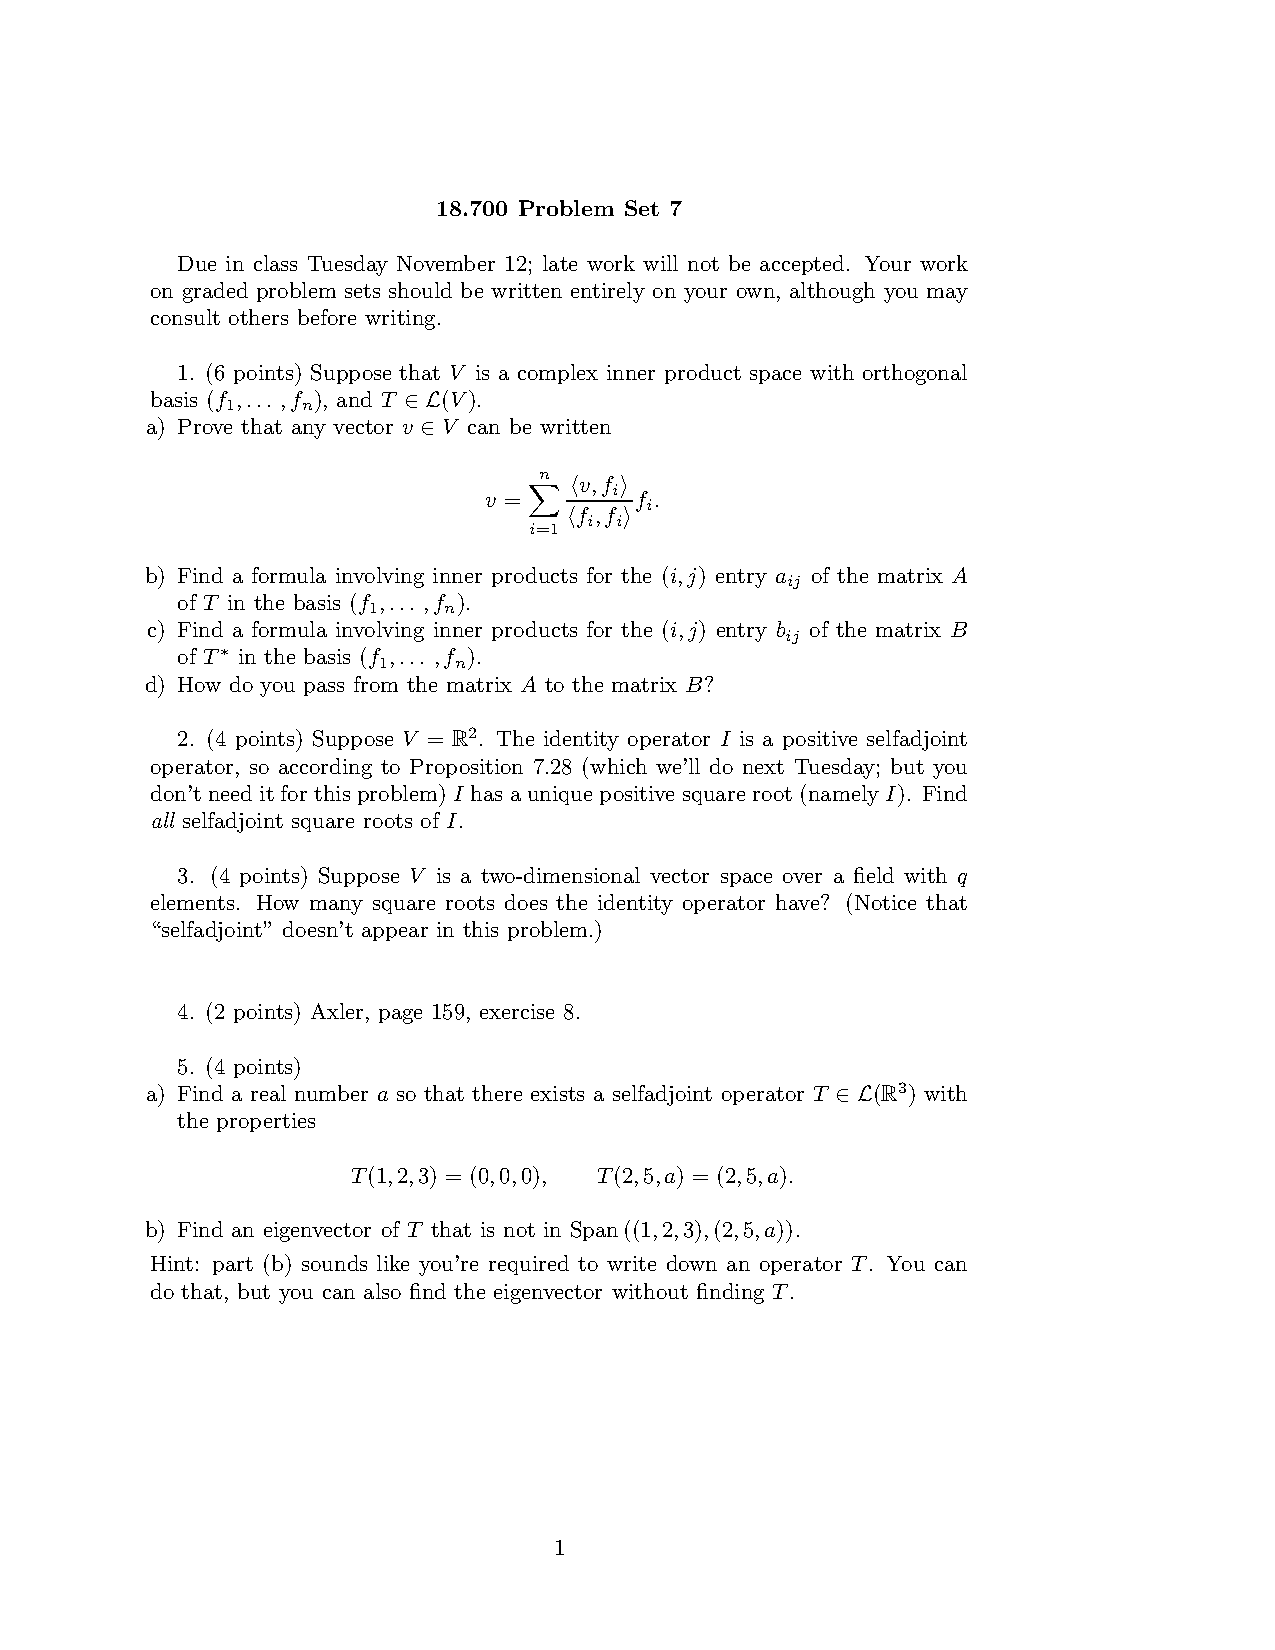
\includepdf[link=true, linkname=LinearAlgebra-ProblemSet7,pages=1]{MIT/Problems/18.700/ProblemSet7.pdf}
\section*{Question 1}
\subsection*{Part a}
Since $ \{ f_1, \cdots f_n \}$ is a basis, any vector $ v $ can be written as a linear combination of them. Taking the inner product and using the orthogonal property, we have:

\begin{eqnarray*}
  v &=& \sum\limits_{i=1}^n c_i f_i \\
  \langle v, f_k \rangle &=& \sum\limits_{i=1}^n c_i \langle f_i f_k \rangle \\
  \langle v, f_k \rangle &=& c_k \langle f_k f_k \rangle \\  
  c_k &=& \frac{\langle v, f_k \rangle}{\langle f_k f_k \rangle } \\
    v &=& \sum\limits_{i=1}^n \frac{\langle v, f_i \rangle}{\langle f_i f_i \rangle } f_i \\
\end{eqnarray*}

\subsection*{Part b}
The basic idea is the the $ j $ column of $ A $ is what $ T(f_j) $ is, so $ A_{ij} $ is really just the coefficient of $ T(f_j) $ corresponding to the $ f_i $, which can be extracted using inner product.

Consider the matrix form of $ T(\sum\limits_{i=1}^n c_i f_i) $. 
\begin{eqnarray*}
  & & T(\sum\limits_{i=1}^n c_i f_i) \\
  &=& \sum\limits_i (\sum\limits_j A_{ij} c_j) f_i
\end{eqnarray*}
Suppose the vector under transformation is $ f_q $, then $ c_i = \delta_{iq} $, we have:

\begin{eqnarray*}
                       T(f_q) &=& \sum\limits_i A_{iq} f_i \\
  \langle T(f_q), f_p \rangle &=& \langle \sum\limits_i A_{iq} f_i, f_p \rangle \\
                              &=& A_{pq}\langle f_p, f_p \rangle \\
                       A_{pq} &=& \frac{\langle T(f_q), f_p \rangle}{\langle f_p, f_p \rangle}
\end{eqnarray*}

\subsection*{Part c}
Similarly, $ B_{ij} $ is the coefficient of $ T^*(f_j)$ corresponding to $ f_i $, so we have a similar calculation here:

\begin{eqnarray*}
                       T^*(f_q) &=& \sum\limits_i B_{iq} f_i \\
  \langle T^*(f_q), f_p \rangle &=& \langle \sum\limits_i B_{iq} f_i, f_p \rangle \\
                                &=& B_{pq}\langle f_p, f_p \rangle \\
                         B_{pq} &=& \frac{\langle T^*(f_q), f_p \rangle}{\langle f_p, f_p \rangle}
\end{eqnarray*}

\subsection*{Part d}
Let's do more simplification of $ B_{pq} $
\begin{eqnarray*}
   B_{pq} &=& \frac{\langle T^*(f_q), f_p \rangle}{\langle f_p, f_p \rangle} \\
          &=& \frac{\langle f_q, T(f_p) \rangle}{\langle f_p, f_p \rangle} \\
          &=& \frac{\overline{\langle T(f_p), f_q \rangle}}{\langle f_p, f_p \rangle}
\end{eqnarray*}
So 
\begin{eqnarray*}
   B_{pq}\langle f_p, f_p \rangle &=& \overline{\langle T(f_p), f_q \rangle} \\
                                  &=& \overline {A_{qp}\langle f_q, f_q \rangle} \\
                           B_{pq} &=& \overline {A_{qp}}\frac{\langle f_q, f_q \rangle}{\langle f_p, f_p \rangle}
\end{eqnarray*}

This would be a simple conjugate transpose if the basis is orthonormal instead of just orthogonal.
\section*{Question 2}
Consider a general self-adjoint square root of $ I \in \mathbf{R}^2 $ as follow:
\begin{eqnarray*}
  \left(\begin{array}{cc}
    a & b \\ 
    b & d 
  \end{array}\right)\left(\begin{array}{cc}
    a & b \\ 
    b & d 
  \end{array}\right) &=& \left(\begin{array}{cc}
    1 & 0 \\ 
    0 & 1 
  \end{array}\right)
\end{eqnarray*}
This boils down to the equations
\begin{eqnarray*}
  a^2 + b^2 = b^2 + d^2 = 1 \\
  b(a + d) = 0 
\end{eqnarray*}
The latter equation is easier to solve, it is either $ b = 0 $ or $ a = -d $ (or both).

In case $ b = 0 $, we have $ a^2 = d^2 = 1 $, so $ a = \pm 1 $ and $ d = \pm 1 $, signs can be chosen arbitrarily.

In case $ a = -d $, $ b = \pm\sqrt{1 - a^2} $ will also satisfy the first equation, this equation only make sense if $ -1 \le a \le 1 $. Notice that when $ a = \pm 1 $, this cover some cases when $ b = 0 $, and that's okay.

This included all self-adjoint square root of $ I $.
\section*{Question 3}
Consider a general square root of $ I \in \mathbf{F_q}^2 $ as follow:
\begin{eqnarray*}
  \left(\begin{array}{cc}
    a & b \\ 
    c & d 
  \end{array}\right)\left(\begin{array}{cc}
    a & b \\ 
    c & d 
  \end{array}\right) &=& \left(\begin{array}{cc}
    1 & 0 \\ 
    0 & 1 
  \end{array}\right)
\end{eqnarray*}
This boils down to the equations
\begin{eqnarray*}
  a^2 + bc = bc + d^2 = 1 \\
  b(a + d) = c(a + d) = 0 
\end{eqnarray*}
The latter equation is easier to solve, it is either $ b = c = 0 $ or $ a = -d $ (or both).

In case $ b = c = 0 $, we have $ a^2 = d^2 = 1 $, so $ a = \pm 1 $ and $ d = \pm 1 $, signs can be chosen arbitrarily.

In case $ a = -d $, $ bc = 1- a^2 $. So it depends on the value of $ 1 - a^2 $. Suppose $ 1 - a^2 = 0 $, either $ b $ or $ c $ must be 0, and the other is arbitrary. Otherwise, $ 1 - a^2 \ne 0 $, we can have an arbitrary non-zero $ b $, and $ c $ has no choice but to be $ b^{-1} (1 - a^2)$

\subsection*{Case 1}
In the case the field $ F $ has characteristic 2. $ a = -a $ for all field elements. So we have exactly 1 solution $ a = d = 1 = -1 $ when $ b = c = 0 $.

The only case for $ 1 - a^2 = 0 $ is when $ a = 1 $. Let's say $ b = 0 $, $ c $ have $ q $ choices, but we must avoid $ c = 0 $ to avoid double counting, that is $ q - 1 $ solutions. Symmetrically, we have $ q - 1 $ solution for $ c = 0 $ case. Together we have $ 2(q - 1) $ solutions.

Last but not least, there are $ q - 1 $ possibility of $ a $ such that $ 1 - a^2 \ne 0 $. For each of these case, $ b $ can be an arbitrary non-zero which has $ q - 1 $ cases, and $ c $ has no choice, so the number of solution of this type is $ (q - 1)^2 $.

Therefore the total number of solutions should be $ 1 + 2(q - 1) + (q - 1)^2 = q^2 $

\subsection*{Case 2}
Otherwise, the field $ F $ does not have characteristic 2, $ a \ne -a $, and therefore we have exactly 4 solution $ a = d = \pm 1 $ when $ b = c = 0 $.

There are two cases $ 1 - a^2 = 0 $ when $ a = \pm 1 $. Let's say $ b = 0 $, $ c $ have $ q $ choices, but we must avoid $ c = 0 $ to avoid double counting, that is $ 2(q - 1) $ solutions. Symmetrically, we have $ 2(q - 1) $ solution for $ c = 0 $ case. Together we have $ 4(q - 1) $ solutions.

Last but not least, there are $ q - 2 $ possibility of $ a $ such that $ 1 - a^2 \ne 0 $. For each of these case, $ b $ can be an arbitrary non-zero which has $ q - 1 $ cases, and $ c $ has no choice, so the number of solution of this type is $ (q - 2)(q - 1) $.

Therefore the total number of solutions should be $ 4 + 4(q - 1) + (q - 2)(q - 1) = q^2 + q + 2 $

The solution is validated using this simple Sage script:
\begin{verbatim}
Field = GF(3)
MatrixOnField = MatrixSpace(Field,2,2)
elements = []
for _,element in enumerate(Field):
  elements.append(element)
count = 0
for a in elements:
  for b in elements:
    for c in elements:
      for d in elements:
        A = MatrixOnField([[a,b],[c,d]])
        if (A * A == MatrixOnField([[1,0],[0,1]])):
          count = count + 1
print(count)
\end{verbatim}
\section*{Question 4}
This is obviously a contradiction.

$ 33 = \langle (1,2,3), (2,5,7) \rangle = \langle (1,2,3), T(2,5,7) \rangle = \langle T(1,2,3), (2,5,7) \rangle = \langle (0,0,0), (2,5,7) \rangle = 0 $

\section*{Question 5}
\subsection*{Part a}
Following the last question, we need to make sure $ \langle (1, 2, 3), (2, 5, a) \rangle = 0 $, that gives $ a = -4 $.

\subsection*{Part b}
Since $ \langle (1, 2, 3), (2, 5, a) \rangle = 0 $, there should be a third vector that is orthogonal to both of them. Once we find it, this can be used as a basis.

We can find the third vector using the reduced echelon form:
\begin{eqnarray*}
  \left(\begin{array}{ccc}
    1 & 2 & 3 \\
    2 & 5 & -4
  \end{array}\right) \to
  \left(\begin{array}{ccc}
    1 & 0 &  23 \\
    0 & 1 & -10
  \end{array}\right) 
\end{eqnarray*}

So we can easily pick $ (-23, 10, 1) $ as the last vector.

We claim that this vector is actually an eigenvector. To show that, let's consider the matrix of the mapping in this basis

\begin{eqnarray*}
\left(\begin{array}{ccc}
0 & 0 & ? \\
0 & 1 & ? \\
0 & 0 & ?
\end{array}\right)
\end{eqnarray*}

By part 1, we know that the matrix of its adjoint should be.

\begin{eqnarray*}
\left(\begin{array}{ccc}
0 & 0 & 0 \\
0 & 1 & 0 \\
? & ? & ?
\end{array}\right)
\end{eqnarray*}

But the operator is self-adjoint, that means the matrix must be:

\begin{eqnarray*}
\left(\begin{array}{ccc}
0 & 0 & 0 \\
0 & 1 & 0 \\
0 & 0 & ?
\end{array}\right)
\end{eqnarray*}

Whatever the last entry is, it must be the case that $ (-23, 10, 1) $ is an eigenvector.


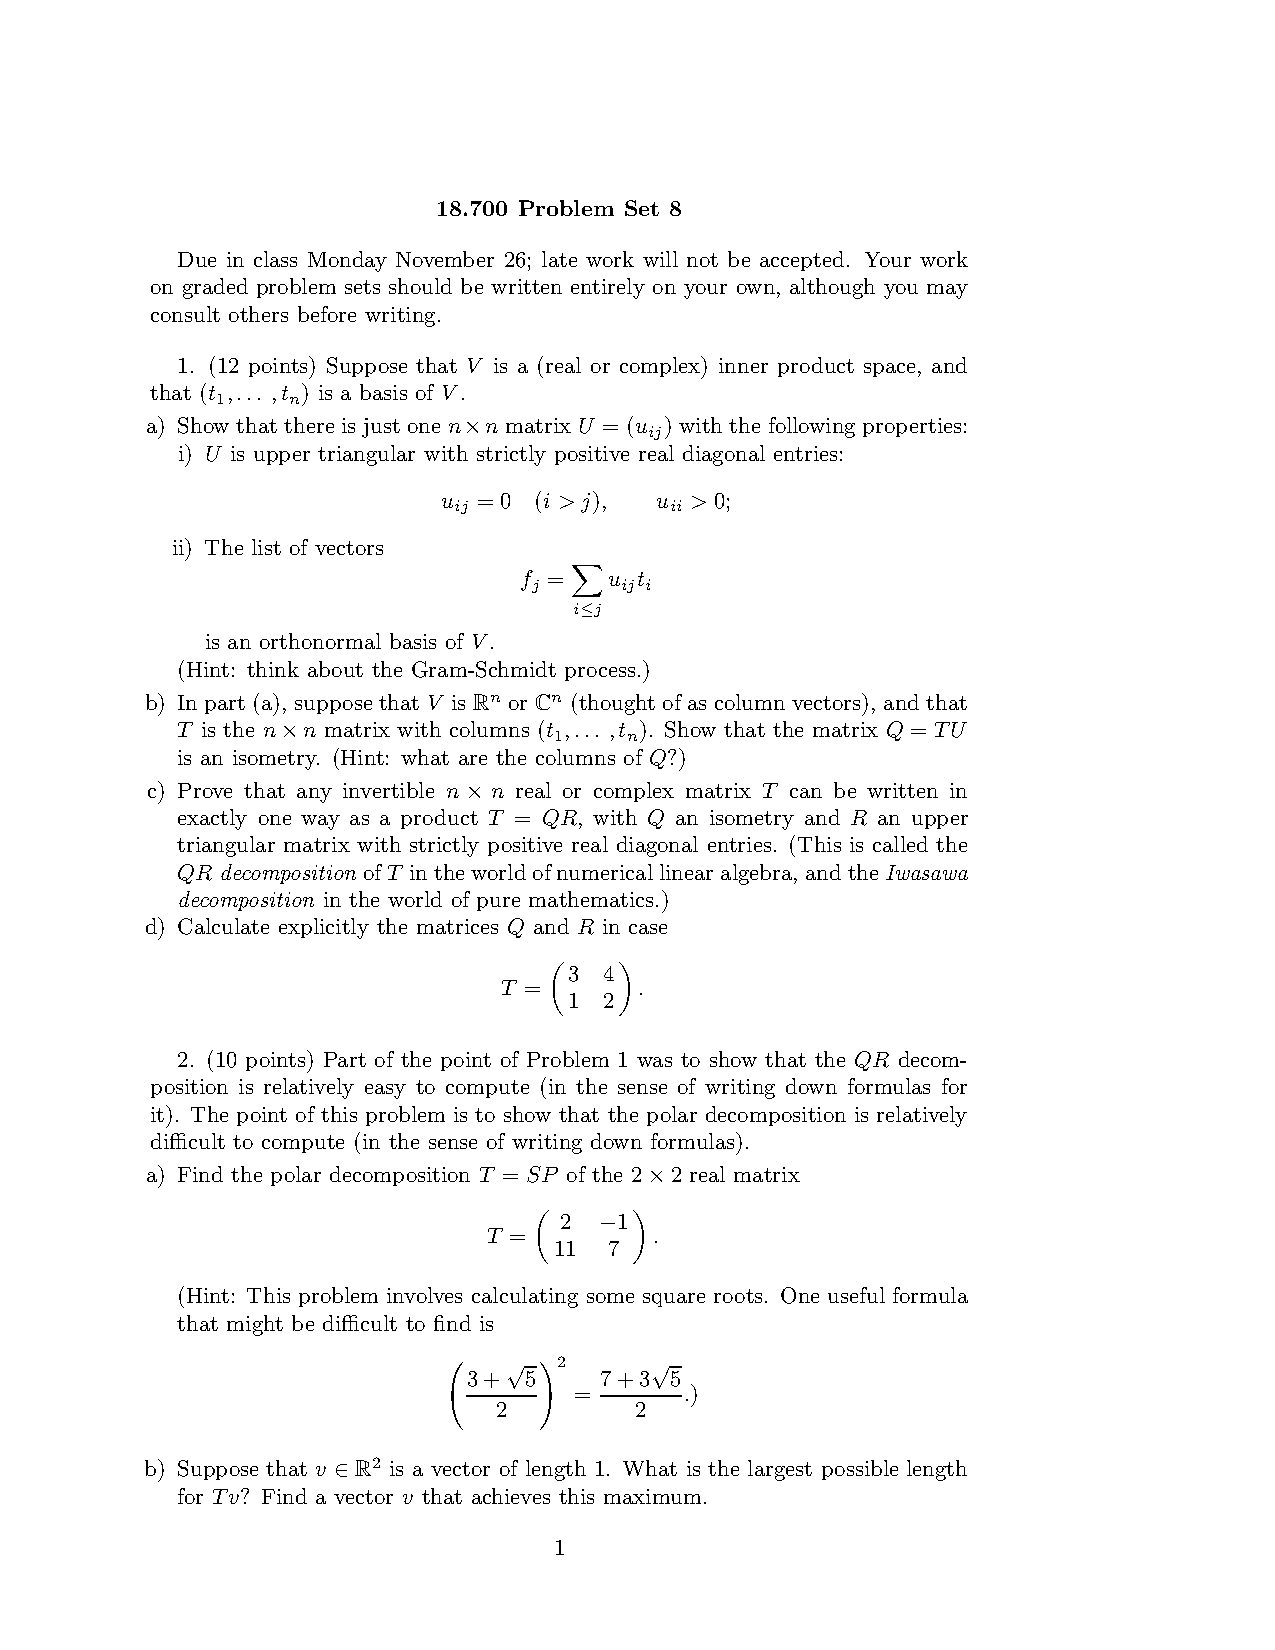
\includepdf[link=true, linkname=LinearAlgebra-ProblemSet8,pages=1]{MIT/Problems/18.700/ProblemSet8.pdf}
\section*{Question 1}
\subsection*{Part a}
We can easily find $ u_{11} $ to be $ \frac{1}{\sqrt{\langle t_1, t_1 \rangle}} $ because $ f_1 = u_{11}t_1 $ must be a unit vector, $ u_{11} > 0 $ because $ \langle t_1, t_1 \rangle > 0 $. Obviously, $ span(f_1) = span(t_1) $.

Assume there exists unique $ u_{ij} $ values such that we can find $ f_1 $ to $ f_k $. Define $ r $ as follow:
\begin{eqnarray*}
  r &=& t_{k+1} - \sum\limits_{j=1}^{k} \langle t_{k+1}, f_j \rangle f_j
\end{eqnarray*}

Now $ r $ is orthogonal to all $ f_1 \cdots f_k $ because for $ 1 \le t \le k $

\begin{eqnarray*}
  & & \langle r, f_t \rangle \\
  &=& \langle t_{k+1}, f_t \rangle - \sum\limits_{j=1}^{k} \langle t_{k+1}, f_j \rangle \langle f_j, f_t \rangle \\
  &=& \langle t_{k+1}, f_t \rangle -  \langle t_{k+1}, f_t \rangle \langle f_t, f_t \rangle \\
  &=& 0
\end{eqnarray*}

So $ r $ is the only direction where it is in the span of $ t_1 \cdots t_{k+1} $ and is also orthogonal to all $ f_1 \cdots f_k $. Since we also have the constraint that $ u_{k+1, k+1} > 0$, therefore the unique $ f_{k+1} $ is given by:

\begin{eqnarray*}
  & & f_{k+1} \\
  &=& \frac{r}{\sqrt{\langle r, r \rangle}} \\
  &=& \frac{1}{\sqrt{\langle r, r \rangle}}(t_{k+1} - \sum\limits_{j=1}^{k} \langle t_{k+1}, f_j \rangle f_j) \\
  &=& \frac{1}{\sqrt{\langle r, r \rangle}}(t_{k+1} - \sum\limits_{j=1}^{k} \langle t_{k+1}, f_j \rangle \sum\limits_{i=1}^{j}u_{ij} t_j)
\end{eqnarray*}

So that proves the existence and uniqueness of the $ u_{ij} $ values.
\subsection*{Part b}
The formula $ f_j = \sum\limits_{i \le j} u_{ij} t_j $ can be rewritten as $ f_j = \sum\limits_{i = 1}^n  t_j u_{ij} $ and that can be interpreted as a block matrix formula as follow:

\begin{eqnarray*}
  (f_1, \cdots f_n) &=& (t_1, \cdots t_n) U \\
                    &=& TU
\end{eqnarray*}

Therefore $ Q $ is the matrix formed by the column vectors of $ f $. We know $ f $ is an orthonormal basis, that means $ Q $ is an othronormal matrix and therefore an isometry.

\subsection*{Part c}
\begin{eqnarray*}
  Q &=& TU \\
  T &=& QU^{-1} 
\end{eqnarray*}

Therefore we need to prove that $ R = U^{-1} $ has the required property (i.e. strictly positive diagonal) and upper triangular.

We already knew $ U $ has such properties, does it carry over to its inverse? The answer is yes, and we can show it using induction as follow:

The upper left $ 1 \times 1 $ submatrix is obviously invertible, and the inverse is a single number that is $ \frac{1}{u_{11}} $ which is strictly positive.

Suppose the upper left $ k \times k $ submatrix is invertible, and now we consider the equation with $ b $ being a scalar and $ b > 0 $

\begin{eqnarray*}
  \left(\begin{array}{cc}
    U_k & a \\
    0   & b
  \end{array}\right)\left(\begin{array}{cc}
    V_k & c \\
    d   & e
  \end{array}\right) &=& \left(\begin{array}{cc}
  I & 0 \\
  0 & 1
  \end{array}\right)
\end{eqnarray*}

We first argue $ d $ must be 0, that is because $ 0 V_k + bd = 0 $. With that $ V_k = U^{-1}_k $, and that's because $ U_kV_k + a 0 = I $, also $ 0 c + b e = 0 $ shows that $ e = \frac{1}{b} > 0 $. Last, but least, $ U_k c+ a e = 0 $, so $ c = - U^{-1}_k ae $ is defined. 

Applying that to the upper left $ k + 1 \times k + 1 $ submatrix, we proved that it is invertible, upper triangular, and the diagonal is also strictly positive.

So by induction, we proved that the inverse of a upper triangular matrix with strictly positive diagonal exists and is also upper triangular with strictly positive diagonal.
\subsection*{Part d}
\begin{eqnarray*}
  & & \langle t_1, t_1 \rangle \\
  &=& 3^2 + 1^2 \\
  &=& 10 \\
  f_1 &=& (\frac{3}{\sqrt{10}},\frac{1}{\sqrt{10}}) \\
  r &=& t_2 - \langle t_2, f_1 \rangle f_1 \\
    &=& (4, 2) - ((4)\frac{3}{\sqrt{10}} + 2\frac{1}{\sqrt{10}}))(\frac{3}{\sqrt{10}},\frac{1}{\sqrt{10}}) \\
    &=& (4, 2) - (\frac{21}{5}. \frac{7}{5}) \\
    &=& (-\frac{1}{5}, \frac{3}{5}) \\
  \langle r, r \rangle &=& (-\frac{1}{5})(-\frac{1}{5}) + (\frac{3}{5})(\frac{3}{5}) \\
    &=& \frac{10}{25} \\
  f_2 &=& \frac{r}{\sqrt{\langle r, r \rangle}} \\
      &=& \frac{(-\frac{1}{5}, \frac{3}{5})}{\sqrt{\frac{10}{25}}} \\
      &=& (\frac{-1}{\sqrt{10}},\frac{3}{\sqrt{10}})
\end{eqnarray*}
The computation of $ f_2 $ is not just tedious, it is also unnecessary, since we already knew $ \langle f_1, f_2 \rangle = 0 $, it would be easy to get $ f_2 $ that way. (But which direction?)

So we have
\begin{eqnarray*}
  Q &=& \frac{1}{\sqrt{10}}\left(\begin{array}{cc}
     3 & -1 \\
     1 & 3 
  \end{array}\right) \\
  R &=& Q^{-1}T \\
  &=& \frac{1}{\sqrt{10}}\left(\begin{array}{cc}
     3 & 1 \\
     -1 & 3 
  \end{array}\right)\left(\begin{array}{cc}
     3 & 4 \\
     1 & 2 
  \end{array}\right) \\
  &=& \frac{1}{\sqrt{10}}\left(\begin{array}{cc}
     10 & 14 \\
     0 & 2
  \end{array}\right)
\end{eqnarray*}

As an aside, the qr routine in Octave does not provide the same answer. It turns out that the qr routine in Octave does not guarantee strictly positive diagonal.
\section*{Question 2}
\subsection*{Part a}
Consider the problem of finding the square root of $ T^* T = \left(\begin{array}{cc} 125 & 75 \\ 75 & 50 \end{array}\right) $ by assuming the square root is $ \left(\begin{array}{cc} x & y \\ y & z \end{array}\right)$. That gives us the equations:

\begin{eqnarray*}
  \left(\begin{array}{cc} x & y \\ y & z \end{array}\right)\left(\begin{array}{cc} x & y \\ y & z \end{array}\right) &=& \left(\begin{array}{cc} 125 & 75 \\ 75 & 50 \end{array}\right)
\end{eqnarray*}

or in an expanded form:
\begin{eqnarray*}
  x^2 + y^2 &=& 125 \\
    xy + yz &=& 75  \\
  y^2 + z^2 &=& 50
\end{eqnarray*}

These equations can be significantly simplified using Gröbner basis. We can find that basis using Sage easily as follows:

\begin{verbatim}
R.<x,y,z> = PolynomialRing(QQ, order='lex')
ideal(x^2 + y^2 - 125, x*y + y*z - 75, y^2 + z^2 - 50).groebner_basis()
\end{verbatim}

This command will give us the basis as:
\begin{eqnarray*}
  x + \frac{1}{10}z^3 - \frac{9}{2}z \\
  y + \frac{1}{10}z^3 - \frac{7}{2}z \\
  z^4 - 30z^2 + 125 
\end{eqnarray*}

Note that the last equation is has root $ \pm 5, \pm \sqrt{5} $ simply solving it as a quadratic equation, and once we know $ z $, it is trivial to compute $ x $ and $ y $. Therefore the roots are:

\begin{eqnarray*}
  x = 10, y = 5, z = 5 \\
  x = 10, y = -5, z = -5 \\
  x = 4\sqrt{5}, y = 3\sqrt{5}, z = 5 \\
  x = -4\sqrt{5}, y = -3\sqrt{5}, z = -5
\end{eqnarray*}

We simply pick the first one for simplicity. Once we know $ R $, we can simply compute $ S = TR^{-1} $ to find the full polar decomposition as :

\begin{eqnarray*}
  T &=& \left(\begin{array}{cc} 2 & -1 \\ 11 & 7 \end{array}\right) \\
    &=& \frac{1}{5}\left(\begin{array}{cc}3 & -4 \\ 4 & 3\end{array}\right)\left(\begin{array}{cc} 10 & 5 \\ 5 & 5 \end{array}\right)
\end{eqnarray*}

\subsection*{Part b}
We know that $ S $ is an isometry, so maximizing $ Tv $ is the same as maximizing $ Rv $, and $ R $ is much simpler. Consider $ v = \left(\begin{array}{c} x \\ y \end{array}\right)$

\begin{eqnarray*}
  |Tv|^2 &=& \left|\left(\begin{array}{cc} 10 & 5 \\ 5 & 5 \end{array}\right)\left(\begin{array}{c} x \\ y \end{array}\right)\right|^2 \\
       &=& \left|\left(\begin{array}{c} 10x + 5y \\ 5x + 5y \end{array}\right)\right|^2 \\
       &=& (10x + 5y)^2 + (5x + 5y)^2 \\
       &=& 125x^2 + 150xy + 50y^2 \\
\end{eqnarray*}

To optimize it, we will use the Lagrangian
\begin{eqnarray*}
  L &=& 125x^2 + 150xy + 50y^2 - \lambda(x^2 + y^2 - 1) \\
  \frac{\partial{L}}{\partial x} &=& 250x + 150y - 2\lambda x = 0 \\
  \frac{\partial{L}}{\partial y} &=& 150x + 100y - 2\lambda y = 0
\end{eqnarray*}

Using Gröbner basis again:
\begin{verbatim}
R.<x,y,z> = PolynomialRing(QQ, order='lex')
ideal(250*x + 150*y - 2*z*x,150*x + 100*y - 2*z*y,x^2+y^2-1).groebner_basis()
\end{verbatim}

We find the equations simplifies as follow:
\begin{eqnarray*}
  x - \frac{yz}{75} + \frac{2y}{3} &=& 0 \\
  y^2 + \frac{z}{375} - \frac{11}{15} &=& 0 \\
  z^2 - 175z + 625 &=& 0 
\end{eqnarray*}

And finally we solve as follows:
\begin{eqnarray*}
  z &=& \frac{25}{2}(7 \pm 3 \sqrt{5}) \\
  y &=& \pm\sqrt{\frac{1}{2}\left(1 \pm \frac{1}{\sqrt{5}}\right)} \\
  x &=& \pm\sqrt{\frac{1}{2}\left(1 \mp \frac{1}{\sqrt{5}}\right)} \\
\end{eqnarray*}

These four solutions correspond to two pairs of vectors, one pair that minimize $ |Tv| $, and one that maximize $ |Tv| $. The solution that maximize $ |Tv| $ is:

\begin{eqnarray*}
  x &=& \sqrt{\frac{1}{2}\left(1 + \frac{1}{\sqrt{5}}\right)} \\
  y &=& \sqrt{\frac{1}{2}\left(1 - \frac{1}{\sqrt{5}}\right)}
\end{eqnarray*}

Last but not least, the maximum length is 
\begin{eqnarray*}
  & & \sqrt{125x^2 + 150xy + 50y^2} \\
  &=& \sqrt{\frac{25}{2} (7 + 3 \sqrt{5})} \\
  &=& 5\sqrt{\frac{7 + 3\sqrt{5}}{2}} \\
  &=& 5\left(\frac{3 + \sqrt{5}}{2}\right)
\end{eqnarray*}

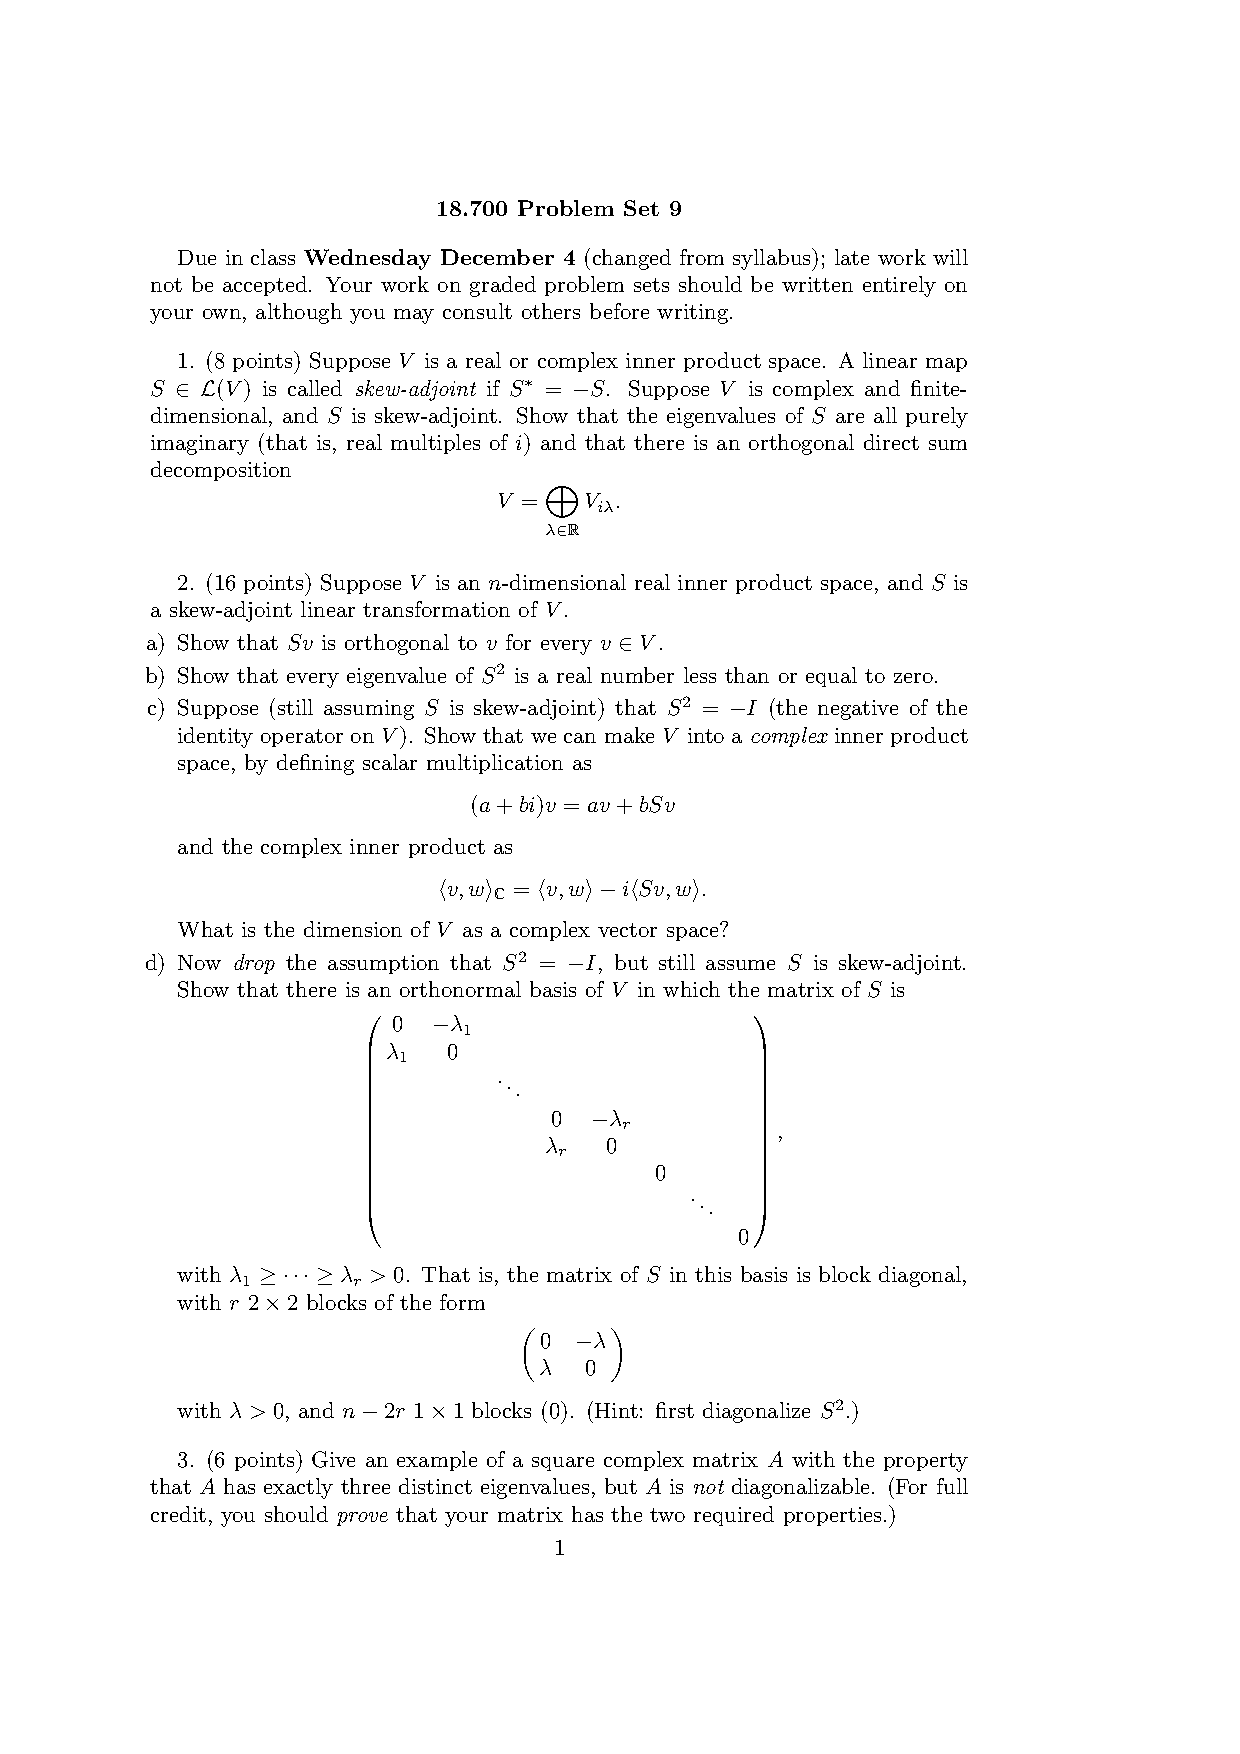
\includepdf[link=true, linkname=LinearAlgebra-ProblemSet9,pages=1]{MIT/Problems/18.700/ProblemSet9.pdf}
\section*{Question 1}
Note that $ SS^* = S^*S = -S^2 $, therefore $ S $ is normal. By the spectral theorem, $ S $ has an orthonormal basis of eigenvectors.

Consider $ \langle Sv , v \rangle $ for a normalized eigenvector $ v $ evaluated in both ways:

\begin{eqnarray*}
  & & \langle Sv , v \rangle      \\
  &=& \langle \lambda v, v \rangle \\
  &=& \lambda \langle v, v \rangle \\
  &=& \lambda 
\end{eqnarray*}

But we can also evaluate it this way:

\begin{eqnarray*}
  & & \langle Sv , v \rangle   \\
  &=& \langle v, S^* v \rangle \\
  &=& \langle v, -Sv \rangle   \\
  &=& \langle v, -\lambda v \rangle   \\
  &=& \overline{ \langle -\lambda v, v \rangle }  \\
  &=& \overline{ -\lambda \langle  v, v \rangle }  \\
  &=& \overline{ -\lambda }  \\
\end{eqnarray*}

This shows that $ \lambda = \overline{-\lambda} $, therefore $ \lambda $ must be purely imaginary. This applies to all eigenvalues.

For each eigenvector $ v_k $, we can have a vector space $ U_k = span(v_k) $, since $ v_k $ form a basis, every vector can be written uniquely as a linear combination of these vectors, i.e. they form a direct sum.
\section*{Question 2}
\subsection*{Part a}
\begin{eqnarray*}
    & & \langle Sv , v \rangle     \\
    &=& \langle v , S^* v \rangle  \\
    &=& \langle v , -Sv \rangle   \\
    &=& \langle -Sv , v \rangle   \\
    &=& - \langle Sv , v \rangle
\end{eqnarray*}
Therefore $ \langle Sv , v \rangle = 0 $.

\subsection*{Part b}
Consider $ v $ to be a normalized eigenvector of $ S^2 $ with eigenvalue $ \lambda $, then
\begin{eqnarray*}
    & & \lambda \\
    &=& \langle \lambda v , v \rangle     \\
    &=& \langle S^2v , v \rangle     \\
    &=& \langle Sv , S^* v \rangle  \\
    &=& \langle Sv , -Sv \rangle   \\
    &=& \langle -Sv , Sv \rangle   \\
    &=& - \langle Sv , Sv \rangle
\end{eqnarray*}

So $ \lambda $ is a real number less than or equal to 0 because $ \langle Sv , Sv \rangle $ is a real number greater than 0 or equal to 0.

\subsection*{Part c}
We will show that the construction leads to a new complex inner product space by showing the axioms holds.

\begin{enumerate}
    \item{ 
        Associativity/Commutativity/Identity/Inverse of vector addition follows from $ V $ since the definition of vector addition is unchanged.
    }
    \item {
        Compatibility of scalar multiplication with field multiplication:
        
        For this purpose, we need to prove $ a(bv) = (ab)v $, we simply evaluate both the left and right hand side.

        For the left hand side, we have:
        \begin{eqnarray*}
          & & a(bv) \\
          &=& (p+qi)((r+si) v) \\
          &=& (p+qi)(r+sS)v \\
          &=& (p+qS)(r+sS)v \\
          &=& (pq + qrS + psS + psS^2)v \\
          &=& ((pr-qs) + (ps+qr)S)v
        \end{eqnarray*}

        On the right hand side, we have:
        \begin{eqnarray*}
          & & (ab)v \\
          &=& ((p+qi)(r+si))v \\
          &=& ((pr-qs)+(ps+qr)i)v \\
          &=& ((pr-qs)+(ps+qr)S)v
        \end{eqnarray*}

        So the left hand side and the right hand side equals and we have the compatibility of scalar multiplication with field multiplication.
    }
    \item {
        Identity element of scalar multiplication:

        For this purpose, we need to prove $ 1v = v $, we simply evaluate.

        \begin{eqnarray*}
          & & 1v \\
          &=& (1+0i)v \\
          &=& v
        \end{eqnarray*}

        So we have the identity element of scalar multiplication
    }
    \item {
        Distributivity of scalar multiplication with respect to vector addition:

        For this purpose, we need to prove $ a(u+v) = au + av $, we simply evaluate both the left and right hand side.
        
        So the left hand side and the right hand side equals and we have the distributivity of scalar multiplication with respect to vector addition.
    }
    \item {
        Distributivity of scalar multiplication with respect to field addition:

        For this purpose, we need to prove $ (a + b)v = av + bv $, we simply evaluate both the left and right hand side.

        For the left hand side, we have:
        \begin{eqnarray*}
          & & ((p+qi)+(r+si))v \\
          &=& ((p+r)+(q+s)i)v \\
          &=& ((p+r)+(q+s)S)v \\
          &=& pv+rv+qSv+sSv
        \end{eqnarray*}

        On the right hand side, we have:
        \begin{eqnarray*}
          &=& (p+qi)v + (r+si)v  \\
          &=& pv+qSv+rv+sSv \\
          &=& pv+rv+qSv+sSv
        \end{eqnarray*}

        So the left hand side and the right hand side equals and we have the distributivity of scalar multiplication with respect to field addition.
    }
\end{enumerate}
At this point, we have verified all the vector space axioms, next, we move on to the inner product space axioms.

\begin{enumerate}
    \item{
        Conjugate symmetry:

        For this purpose, we need to prove $ \langle x, y\rangle_\mathbf{C} = \overline{\langle y, x\rangle}_\mathbf{C}$, we simply evaluate both the left and right hand side.

         For the left hand side, we have:
        \begin{eqnarray*}
          & & \langle x, y\rangle_\mathbf{C} \\
          &=& \langle x, y\rangle - i \langle Sx, y\rangle
        \end{eqnarray*}

        On the right hand side, we have:
        \begin{eqnarray*}
          &=& \overline{\langle y, x\rangle}_\mathbf{C} \\
          &=& \overline{\langle y, x\rangle - i \langle Sy, x\rangle} \\
          &=& \langle y, x\rangle + i \langle Sy, x\rangle \\
          &=& \langle y, x\rangle - i \langle y, Sx\rangle \\
          &=& \langle x, y\rangle - i \langle Sx, y\rangle
        \end{eqnarray*}

        So the left hand side and the right hand side equals and we have the conjugate symmetry.
    }
    \item{
        Linearity in the first argument:

        For this purpose, we need to prove $ \langle ax+by, z\rangle_\mathbf{C} = a\langle x, z\rangle_\mathbf{C} + b\langle y, z\rangle_\mathbf{C} $, we simply evaluate both the left and right hand side.

         For the left hand side, we have:
        \begin{eqnarray*}
          & & \langle ax + by, z\rangle_\mathbf{C} \\
          &=& \langle ax + by, z\rangle - i \langle S(ax+by), z\rangle \\
          &=& a\langle x, z\rangle + b\langle y, z\rangle - i a\langle Sx, z\rangle - i b\langle Sy, z\rangle
        \end{eqnarray*}

        On the right hand side, we have:
        \begin{eqnarray*}
          &=& a\langle x, z\rangle_\mathbf{C} + b\langle y, z\rangle_\mathbf{C} \\
          &=& a(\langle x, z\rangle - i \langle Sx, z\rangle) + b(\langle y, z\rangle - i \langle Sy, z\rangle) \\
          &=& a\langle x, z\rangle + b\langle y, z\rangle - i a\langle Sx, z\rangle - i b\langle Sy, z\rangle
        \end{eqnarray*}

        So the left hand side and the right hand side equals and we have the linearity in the first argument.
    }
    \item{
        Positive-definiteness:

        For this purpose, we need to prove $ \langle x, x\rangle_\mathbf{C} > 0 $ if $ x \ne 0 $

        \begin{eqnarray*}
          & & \langle x, x\rangle_\mathbf{C} \\
          &=& \langle x, x\rangle - i \langle Sx, x\rangle \\
          &=& \langle x, x\rangle \\
          &>& 0
        \end{eqnarray*}

        So we have positive definiteness.
    }
\end{enumerate}

Now we have proved that the new multiplication rule and inner product rule make $ V $ complex inner product space.

To study the dimension of the new complex vector space, we first note that $ (S^2)^* = (S^*)^2 = (-S)^2 = S^2 $, so $ S^2 $ is self-adjoint. By the spectral theorem we know that $ S^2 $ can be diagonalized with an orthonormal basis of $ V $.

Suppose $ S^2 v = \lambda v $ for $ \lambda \ne 0$, $ v \ne 0 $, we have $ S^2(Sv) = S(S^2v) = S \lambda v 
 = \lambda Sv $, so $ Sv $ is also an eigenvector of $ S^2 $ with the same eigenvalue. Furthermore, as we proved in part (a), $ v $ and $ Sv $ are orthogonal. We claim that the eigenspaces of $ S^2 $ with non-zero eigenvalue can always be spanned by some $ v $ and $ Sv $ pairs which are mutually orthogonal.

We already proved that $ v $ and $ Sv $ are there, suppose (for the purpose of induction) that we have already found $ v_1,  Sv_1 \cdots v_k, Sv_k $ and that that still doesn't span the whole eigenspace. Now can extend the basis to find $ v_{k+1} $ so that it is orthogonal to all of them and consider $ Sv_{k+1} $.

First or all, we know $ Sv_{k+1} $ is also an eigenvector of $ S^2 $ with the same eigenvalue. Next, $ Sv_{k+1} $ is orthogonal to $ v_{k+1} $ by part (a). Also, for any $ 1 \le i \le k $ we have these orthogonality relations.

\begin{eqnarray*}
  & & \langle Sv_{k+1}, v_i \rangle \\
  &=& \langle v_{k+1}, S^* v_i \rangle \\
  &=& -\langle v_{k+1}, S v_i \rangle \\
  &=& 0
\end{eqnarray*}


\begin{eqnarray*}
  & & \langle Sv_{k+1}, Sv_i \rangle \\
  &=& \langle v_{k+1}, S^*S v_i \rangle \\
  &=& \langle v_{k+1}, -S^2 v_i \rangle \\
  &=& -\lambda \langle v_{k+1}, v_i \rangle \\
  &=& 0
\end{eqnarray*}

Therefore $ Sv_{k+1} $ is orthogonal to every earlier vectors, and therefore we can extend the basis by one more pair. By the principle of induction, we know that the eigenspace can be spanned by mutually orthogonal pairs.

Note carefully that this fact is independent of the fact that $ S^2 = -I $, this is going to be useful for part (d).

Since $ S^2 = -I $, $ S^2 $ is injective, so is $ S $, therefore $ Sv \ne 0 $ if $ v \ne 0 $, that means 0 is not an eigenvalue of $ S $. 

Therefore the whole vector space V is spanned by the $ v, Sv $ pairs. Therefore $ N $, the dimension of $ V $ must be an even number.

Last but not least, we claim that the dimension of the new complex vector space is $ \frac{N}{2} $, this can be seen by picking the $ v $ of the $ v, Sv $ pair basis By multiplying with a pure imaginary number will get us the $ Sv $ part of it. We also know the together they span the whole space. Knowing that the $ v, Sv $ pairs are all mutually orthogonal, we also know that these vectors are mutually orthogonal in the new complex vector space, therefore we have found the $ \frac{N}{2} $ orthogonal basis vectors.

\subsection*{Part d}
The earlier problem shows that eigenspaces of non-zero eigenvalues can be spanned by $ v, Sv $ pairs. Now, without the $ S^2 = -I $ constraint, 0 could be an eigenvalue for eigenvector $ v $. In that case, we might have

\begin{eqnarray*}
  & & \langle Sv, Sv \rangle \\
  &=& \langle v, S^*Sv \rangle \\
  &=& -\langle v, S^2v \rangle \\
  &=& -\langle v, 0 \rangle \\
  &=& 0
\end{eqnarray*}

So $ v $ is also an eigenvector of $ S $ with eigenvalue 0.

This gives us all the ingredients we need. To pick the basis, for each non-zero eigenvalue $ -\lambda^2 $ with eigenvector pair $ v, Sv $, we choose $ \lambda v $ and $ Sv $ to be the basis. Transforming them with $ S $ give us $ S \lambda v = \lambda Sv $ and $ S(Sv) = S^2 v = -\lambda^2 v = -\lambda (\lambda v) $. This fits exactly with what we needed in the matrix.

We also know that the eigenvectors with zero eigenvalues are also eigenvector of $ S $, so we can simply stick them at the end.

Last but not least, since these are eigenvectors of $ S^2 $, we already knew they are orthogonal. To make it orthonormal, note that $ \langle Sv, Sv \rangle = \langle v, -S^2v \rangle = \lambda^2 \langle v, v \rangle = \langle \lambda v, \lambda v \rangle $, so all we need to do is to normalize the $ v $ such that $ \langle v, v \rangle = \frac{1}{\lambda} $, the $ Sv $ will be automatically normalized to 1, and we can also pick the eigenvectors of zero eigenvalue to be unit length, and now we get the orthonormal basis.

\section*{Question 3}
This matrix has the required property:
\begin{eqnarray*}
    A = \left(\begin{array}{cccc}
      1 & 1 & 0 & 0 \\
      0 & 1 & 0 & 0 \\
      0 & 0 & 2 & 0 \\
      0 & 0 & 0 & 3
    \end{array}\right)
\end{eqnarray*}
Obviously, 1, 2, 3 are the three distinct eigenvalues of it, and we cannot diagonalize it because the null space of $ A - I $ has only one dimension, therefore the dimension of the eigenspace is insufficient to form the basis.


\fi

%
% Modern Algebra
%
\pagebreak
\section*{Problem Set 1}
\hypertarget{ModernAlgebra-Assignment01}{}

\begin{enumerate}
    \item{Ex 2: 1-4, 7-10, 12}
    \item{Ex 4: 1-6, 12, 14, 20}
    \item{Ex 5: 1-3, 13, 20}
    \item{Ex 6: 4, 17, 19, 21, 22, 28, 32, 33, 34}
\end{enumerate}

Bonus problems:
\begin{enumerate}
    \item{If associativity of 3 factors holds, then prove that a*b*c*d is independent of the way one puts parentheses.}
    \item{Prove that $ bij(S) $ is commutative if and only if $ |S| $ = $ 1 $ or $ 2 $.}
\end{enumerate}




\includepdf[pages=2-3]{MIT/Problems/18.703/fraleigh-excerpts.pdf}

\section*{Ex2 - 1}
\begin{enumerate}
    \item{$ b * d = e $ }
    \item{$ c * c = b $ }
    \item{$ [(a * c) * e] * a = [c * e] * a = a * a = a $ }
\end{enumerate}
\section*{Ex2 - 2}
We have $ (a * b) * c = b * c = a $ and $ a * (b * c) = a * a = a $. That looks like associative, but associativity requires that it works for all triples, we cannot confirm associativity with just one example.
\section*{Ex2 - 3}
We have $ (b * d) * c = e * c = a $ and $ b * (d * c) = b * b = c $. That confirms the operation $ * $ is not associative.
\section*{Ex2 - 4}
$ * $ is commutative because the multiplication table is symmetric about the diagonal.
\section*{Ex2 - 7}
We have $ 1 - 2 \ne 2 - 1 $, therefore the operation is not commutative.

$ -4 = (1 - 2) - 3\ne 1 - (2 - 3) = 2 $, therefore the operation is not associative.


\section*{Ex2 - 8}
$ ab = ba $ for all $ a, b \in \mathbb{Q} $, therefore $ ab + 1 = ba + 1 $ and the operation is commutative.

For associativity, we have $ (a * b) * c = (ab + 1)c + 1 = abc + c + 1 $ and $ a * (b * c) = a(bc + 1) + 1 = abc + a + 1 $. So when $ a \ne c $, the two sides are not equal, and the operation is not associative.
\section*{Ex2 - 9}
$ ab = ba $ for all $ a, b \in \mathbb{Q} $, therefore $ \frac{ab}{2} = \frac{ba}{2} $ and the operation is commutative.

Also, $ (a * b) * c = \frac{\frac{ab}{2}c}{2} = \frac{abc}{4} = \frac{a\frac{bc}{2}}{2} = a * (b * c) $. So the operation is associative.
\section*{Ex2 - 10}
$ ab = ba $ for all $ a, b \in \mathbb{Z}^+ $, therefore $ 2^{ab} = 2^{ba} $ and the operation is commutative.

$ (1 * 2) * 3  = 2^2 * 3 = 2^{12} $ and $ 1 * (2 * 3) = 1 * 2^6 = 2^{64} $. So the operation is not associative.
\section*{Ex2 - 12}
\begin{enumerate}
\item{If $ S $ has only one element, say, $ e $, we can only define $ e * e = e $, so there is only one binary operations.}
\item{If $ S $ has only two elements, the multiplication table have 4 cells, without any further restriction, each of these cells has 2 options, therefore we have $ 2^4 = 16 $ possible binary operations.}
\item{If $ S $ has only three elements, the multiplication table have 9 cells, without any further restriction, each of these cells has 2 options, therefore we have $ 3^9 = 19683 $ possible binary operations.}
\item{If $ S $ has only $ n $ elements, the multiplication table have $ n^2 $ cells, without any further restriction, each of these cells has 2 options, therefore we have $ n^(n^2) $ possible binary operations.}
\end{enumerate}

Just as a comment - there could be $ 4^16 = 4294967296 $ binary operations on 4 elements, but there are only 2 non-isomorphic groups of order 4.

\includepdf[pages=4-5]{MIT/Problems/18.703/fraleigh-excerpts.pdf}

\section*{Ex4 - 1}
$ * $ does not give a group structure on $ \mathbb{Z} $ because $ \mathscr{G}_3 $ does not hold, 2 does not have an inverse element. 
\section*{Ex4 - 2}
$ * $ does give a group structure on $ 2\mathbb{Z} $
\begin{enumerate}
    \item {$ \mathscr{G}_1 $ holds because addition is associative}
    \item {$ \mathscr{G}_2 $ holds because $ 0 \in 2\mathbb{Z} $ is the identity element}
    \item {$ \mathscr{G}_3 $ holds because for any $ x \in 2\mathbb{Z} $, $ -x \in 2\mathbb{Z} $ is the inverse element of $ x $.}
\end{enumerate}
\section*{Ex4 - 3}
$ * $ does not give a group structure on $ \mathbb{R}^+ $ because $ \mathscr{G}_1 $ does not hold, $ \sqrt{\sqrt{2\times3} \times 4} \ne \sqrt{2 \times \sqrt{3 \times 4}} $ and so $ * $ is not associative.
\section*{Ex4 - 4}
$ * $ does give a group structure on $ \mathbb{Q} $
\begin{enumerate}
    \item {$ \mathscr{G}_1 $ holds because multiplication is associative}
    \item {$ \mathscr{G}_2 $ holds because $ 1 \in \mathbb{Q} $ is the identity element}
    \item {$ \mathscr{G}_3 $ holds because for any $ x \in \mathbb{Q} $, $ \frac{1}{x} \in \mathbb{Q} $ is the inverse element of $ x $.}
\end{enumerate}
\section*{Ex4 - 5}
$ * $ does not give a group structure on $ \mathbb{R}^* $ because $ \mathscr{G}_1 $ does not hold, $ \frac{\frac{2}{3}}{4} \ne \frac{2}{\frac{3}{4}} $ and so $ * $ is not associative.
\section*{Ex4 - 6}
$ * $ does not give a group structure on $ \mathbb{C} $ because $ \mathscr{G}_2 $ does not hold. Since $ a * b $ is real for all $ a, b \in C $, there cannot be an element of $ e \in C $ such that $ (1 + i) * e = (1 + i) $.
\section*{Ex4 - 12}
All $ n \times n $ diagonal matrix under matrix multiplication is not a group because the zero matrix does not have an inverse.
\section*{Ex4 - 14}
All $ n \times n $ diagonal matrix with all diagonal entries 1 or -1 under matrix multiplication is a group.
\begin{enumerate}
    \item {$ \mathscr{G}_1 $ holds because multiplication is associative}
    \item {$ \mathscr{G}_2 $ holds because $ I $ is the identity element}
    \item {$ \mathscr{G}_3 $ holds because for any $ x \in \mathbb{Q} $, $ x $ is the inverse element of $ x $.}
\end{enumerate}
\section*{Ex4 - 20}
To begin with, here is table 4.22 with empty cells annotated with capital letters so that I can refer to them later.

\begin{tabular}{ c|c|c|c|c }
      & e & a & b & c \\
    \hline
    e & e & a & b & c \\
    a & a & P & Q & R \\
    b & b & S & T & U \\
    c & c & V & W & X 
\end{tabular}

Note that in order to have multiplicative inverse, each row and each column must not have duplicated elements, we will use this rule repeatedly.

Following the problem statement, we will first try set $ P = e $. That leave us with $ \{Q, R\} = \{b, c\} $, but then $ Q \ne b $ because that would create a duplicate in the $ b $ column. So $ Q = c $, $ R = b $. Similar reasoning leads to $ S = c $, $ V = b $. Now the table becomes this.

\begin{tabular}{ c|c|c|c|c }
    & e & a & b & c \\
  \hline
  e & e & a & b & c \\
  a & a & e & c & b \\
  b & b & c & T & U \\
  c & c & b & W & X 
\end{tabular}

Now we could have either $ T = a $ or $ T = e $, this leads to these complete tables $ G1 $ and $ G2 $.

G1

\begin{tabular}{ c|c|c|c|c }
    & e & a & b & c \\
  \hline
  e & e & a & b & c \\
  a & a & e & c & b \\
  b & b & c & a & e \\
  c & c & b & e & a 
\end{tabular}

G2

\begin{tabular}{ c|c|c|c|c }
    & e & a & b & c \\
  \hline
  e & e & a & b & c \\
  a & a & e & c & b \\
  b & b & c & e & a \\
  c & c & b & a & e 
\end{tabular}

Alternatively, we could have set $ P = b $ instead, following the same logic, we will reach this table $ G3 $.

G3

\begin{tabular}{ c|c|c|c|c }
    & e & a & b & c \\
  \hline
  e & e & a & b & c \\
  a & a & b & c & e \\
  b & b & c & e & a \\
  c & c & e & a & b 
\end{tabular}

Note that $ G2 $ has a unique property that every element is an inverse of itself, so it cannot be isomorphic with $ G1 $ or $ G3 $. On the other hand, if we swap $ a $ and $ b $ in $ G1 $, then it becomes $ G3 $, so $ G1 $ and $ G3 $ are isomorphic.

Note that at this point we only listed these are the only possible groups, we haven't verified for associativity yet.

\subsection*{Part a}
Yes, all groups of order 4 are commutative.

\subsection*{Part b}
$ G3 $ is isomorphic to $ U4 $ by mapping $ e, a, b, c $ to $ 1, i, -1, -i $ respectively. We also know $ G1 $ is isomorphic to $ G3 $, so $ G1 $ is also isomorphic to $ U4 $.

\subsection*{Part c}
$ G2 $ is isomorphic to the group of diagonal matrix of size $ 2 \times 2 $ with $ 1 $ and $ -1 $ only on the diagonal as follows:

\begin{eqnarray*}
    e = \left(\begin{array}{cc} 1 & 0 \\ 0 & 1 \end{array}\right) \\
    a = \left(\begin{array}{cc} -1 & 0 \\ 0 & 1 \end{array}\right) \\
    b = \left(\begin{array}{cc} 1 & 0 \\ 0 & -1 \end{array}\right) \\
    c = \left(\begin{array}{cc} -1 & 0 \\ 0 & -1 \end{array}\right)
\end{eqnarray*}

Now we have proved that there are two non-isomorphic groups of order 4. Both of them are Abelian.


\includepdf[pages=6-7]{MIT/Problems/18.703/fraleigh-excerpts.pdf}

\section*{Ex5 - 1}

$ \mathbb{R} $ is a subgroup of the group $ \mathbb{C} $ under addition because for all element $ a,b \in \mathbb{R} $, $ a - b \in \mathbb{R} $.
\section*{Ex5 - 2}

$ \mathbb{Q}^+ $ is a not subgroup of the group $ \mathbb{C} $ under addition because $ -1 \notin \mathbb{Q}^+ $.
\section*{Ex5 - 3}

$ 7\mathbb{Z} $ is a subgroup of the group $ \mathbb{C} $ under addition because for all element $ a,b \in 7\mathbb{Z} $, $ a - b \in 7\mathbb{Z} $.
\section*{Ex5 - 13}
The set of $ n \times n $ orthogonal matrix is a subgroup of $ GL(n) $ because if $ A, B $ are orthogonal matrices, then $ (AB^{-1})^TAB^{-1} = (AB^T)^TAB^T = BA^TAB^T = BB^T = I $, showing $ AB^{-1} $ is also an orthogonal matrix.

\section*{Ex5 - 20}
A group $ G_a $ can be a subgroup of another group $ G_b $ if and only if 
\begin{enumerate} 
    \item{$ G_a $ is a subset of $ G_b $, and}
    \item{$ G_a $ and $ G_b $ share the same group operation.}
\end{enumerate} 

First, consider addition, we have this chain.

\begin{eqnarray*}
    G_2 \subset G_8 \subset G_7 \subset G_1 \subset G_4
\end{eqnarray*}

For multiplication, we have two chains

\begin{eqnarray*}
    G_6 \subset G_5
\end{eqnarray*}

and also
\begin{eqnarray*}
    G_9 \subset G_3 \subset G_5
\end{eqnarray*}

The subset relation is reflexive, transistive, therefore the full set of subgroup relationship is the reflexive transitive closure of these subset relationships.


\includepdf[pages=8-9]{MIT/Problems/18.703/fraleigh-excerpts.pdf}

\section*{Ex6 - 4}

When 50 is divided by 8, the quotient is 6 and the remainder is 2.
\section*{Ex6 - 17}

By the Bézout's identity, we have $ 25 \times 5 - 30 \times 4 = 5 $, which means $ 5 $ is an element of the cyclic subgroup generated by 25 in $ \mathbb{Z}_{30} $. Now all multiples of 5 are included in that group, and any element of that group must be a multiple of 5 because all linear combinations of $ 25 $ and $ 30 $ must be a multiple of 5. Now, we know that group has 6 elements: $ \{0, 5, 10, 15, 20, 25\} $.
\section*{Ex6 - 19}

We simply list the elements to be $ \{1, i, -1, -i \} $.
\section*{Ex6 - 21}

We note that $ (1 + i)^4 = -4 $, therefore we have all powers of $ -4 $. In other words, this group has infinitely many elements. Since all elements can be represented as a power of $ (1 + i) $, we can map the elements to $ \mathbb{Z} $, in other words, the group is countable.
\section*{Ex6 - 22}
Since $ \mathbb{Z}_{12} $ is cyclic (generated by 1), each factor $ n < 12 $ generates a cyclic subgroup that is not the same as $ G $. Now we can list all of them.

\begin{eqnarray*}
  G_1 &=& \{0,1,2,3,4,5,6,7,8,9,10,11\} \\
  G_2 &=& \{0,2,4,6,8,10\} \\
  G_3 &=& \{0,3,6,9\} \\
  G_4 &=& \{0,4,8\} \\
  G_5 &=& \{0,6\} \\
  G_6 &=& \{0\}
\end{eqnarray*}

\begin{verbatim}
  digraph G {
    "G1" -> "G2"
    "G1" -> "G3"
    "G2" -> "G4"
    "G2" -> "G5"
    "G3" -> "G5"
    "G4" -> "G6"
    "G5" -> "G6"
  }  
\end{verbatim}

\section*{Ex6 - 28}
Since $ Z_{20} $ is cyclic, we have exactly one subgroup for each factor of its order, therefore the subgroup orders are {1, 2, 4, 5, 10, 20}.  
\section*{Ex6 - 32}

\begin{enumerate}
    \item {Every cyclic group is Abelian. True, because every cyclic group is isomorphic to either $ \mathbb{Z} $ or $ \mathbb{Z}_n $ for some $ n \ge 2 \in \mathbb{N} $ and these groups are Abelian}.
    \item {Every Abelian group is cyclic. False, because $ \mathbb{Z}_2 \oplus \mathbb{Z}_2 $ is not cyclic.}
    \item {$ \mathbb{Q} $ under addition is a cyclic group. False, because if $ \mathbb{Q} $ were cyclic, then it has a generator $ \frac{p}{q} $, but then it cannot generate $ \frac{p}{2q} $.}
    \item {Every element of every cyclic group generate the group. False, the identity element always only generate itself, so unless the group is $ \{0\} $, it never generates the group.}
    \item {There is at least one Abelian group for every finite order $ > 0 $. True, $ \mathbb{Z}_n $ is such a group.}
    \item {Every group with order $ \le 4 $ is cyclic. False, $ \mathbb{Z}_2 \oplus \mathbb{Z}_2 $ is not cyclic.}
    \item {All generators of $ \mathbb{Z}_{20} $ is a prime number. False, 9 generates $ \mathbb{Z}_{20} $.}
    \item {If $ G $ and $ G' $ are groups, then $ G \cap G' $ is a group. False, it isn't even clear which operation to use.}
    \item {If $ H $ and $ K $ are subgroups of a group $ G $, then $ H \cap K $ is a group. True - for each pair of elements $ i, j \in H \cap K $, so $ j^{-1} \in H \cap K $, $ ij^{-1} \in H \cap K $.}
    \item {Every cyclic group of order $ > 2 $ has at two distinct generators. True, for any cyclic group with generator $ g $, $ g^{-1} $ is also a generator. Now if $ g = g^{-1} $, we will have $ g^2 = 1 $ and that contradicts with the fact that the group has order $ > 2 $. Therefore we have at least two distinct generators. }
\end{enumerate}
\section*{Ex6 - 33}
$ \mathbb{Z}_2 \oplus \mathbb{Z}_2 $ is not cyclic.
\section*{Ex6 - 34}
$ \mathbb{Q} $ under addition is an infinite group that is not a cyclic group.

\section*{Bonus-1}
In this problem, I will assume the reader is familiar with the concept of parse trees for expressions. The statement that an expression is independent of the way of placing parenthesis is the same as any expression evaluate the same as if the expression is evaluated left to right, in another words, the parse tree never expands on the right.

The transformation $ p * (q * r) = (p * q) * r $ can be interpreted as reducing the size of the right subtree of the parse tree of the expression.

Now we can proceed to prove by induction that every expression of length $ n $ can be transformed so that it only expand on the left. The case for $ n = 1 $ or $ n = 2 $ is obvious. The case for $ n = 3 $ is given by the associative rule. Assume it is true for $ n = k $, For any expression of length $ k + 1 $, we can use the associative rule to reduce the size of the right subtree, we can keep doing that until the size become 1, then we can use our induction hypothesis to show that the whole expression can be transformed such that it open expands on the left.

This proves that all expression with any length can be evaluated left to right, of course that include the case for just 4 variables.



\section*{Bonus-2}
The case for $ |S| = 1 $ or $ |S| = 2 $ is obvious. The only case I wanted to show is when $ |S| > 2 $, then it is not commutative.

When $ |S| > 2 $, there are at least three elements of $ S $, let's call them $ a $, $ b $, $ c $. These two mappings are not commutative.

\begin{eqnarray*}
    f(a) &=& b \\
    f(b) &=& a \\
    f(x) &=& x \forall x \ne a, x \ne b
\end{eqnarray*}

\begin{eqnarray*}
    g(b) &=& c \\
    g(c) &=& b \\
    g(x) &=& x \forall x \ne b, x \ne c
\end{eqnarray*}

\begin{eqnarray*}
    f(g(a)) &=& f(a) = b \\
    g(f(a)) &=& g(b) = c
\end{eqnarray*}

\pagebreak
\section*{Problem Set 2}
\hypertarget{ModernAlgebra-Assignment02}{}

\begin{enumerate}
    \item{Ex 6: 38, 41, 46, 48, 55}
    \item{Ex 7: 1, 3, 5, 6}
    \item{Ex 8: 2, 8, 10, 17, 23, 26, 30}
    \item{Ex 9: 1, 10, 14}
\end{enumerate}

Bonus problems:
\begin{enumerate}
    \item{Find all continuous isomorphisms: $ (R,+) --> (R_>0,x) $}
    \item{Classify upto an isomorphism, all groups order 1, 2, 3 and 4 the cyclic group usually denoted by $ C_n $ (or order n), show that for $ n \ge 1 $, there is a group of order n. Show that for $ n = 1, 2, 3 $ there are no other groups of order but for $ n = 4 $ there is just one non-ismorphic to $ C_4 $.}
    \item{Find an algorithm for determining the $ k $ of the Chinese Remainder Theorem, other than just checking all numbers between zero and the product of all $ m_i $ where i goes from $ 1 $ to $ n $.}
    \item{Show if two cycles intersect then they do not commute.}
    \item{Find the subgroup of $ S_4 $ which is the group of symmetries of the regular tetrahedron.}
\end{enumerate}


\includepdf[pages=9-10]{MIT/Problems/18.703/fraleigh-excerpts.pdf}

\section*{Ex6 - 38}
The 4th roots of unity are $ e^{\frac{2k\pi i}{4}} $. The primitive 4th roots of unity are $ e^{\frac{(2 \times 1) \pi i}{4}} = i $ and $ e^{\frac{(2 \times 3)\pi i}{4}} = -i $.

\section*{Ex6 - 41}
The 8th roots of unity are $ e^{\frac{2k\pi}{8}} $. The primitive 8th roots of unity are $ e^{\frac{(2 \times 1) \pi i}{8}} = \frac{1}{\sqrt{2}}( 1 + i) $, $ e^{\frac{(2 \times 3) \pi i}{8}} = \frac{1}{\sqrt{2}}(-1 + i) $, $ e^{\frac{(2 \times 5) \pi i}{8}} = \frac{1}{\sqrt{2}}(-1 - i) $ and $ e^{\frac{(2 \times 7) \pi i}{8}} = \frac{1}{\sqrt{2}}( 1 - i) $.
\section*{Ex6 - 46}
$ (ab)^k = a^{-1}(ab)^ka = (ba)^k $.

Therefore the order of $ ba $, the least integer $ n $ such that $ (ba)^n = 1 $, is the same as the order of $ ab $.
\section*{Ex6 - 48}
Let $ G $ be an infinite group, consider all the cyclic subgroup generated by each element of $ g $. Some of them could be the same group, so in general we may have either an infinite number of them or a finite number of them. Let's prove that it is impossible to have just a finite number of them.

Suppose the contrary that we only have a finite number of cyclic subgroups. We knew that the union of these cyclic subgroups is $ G $, so at least one of these cyclic subgroups $ H $, generated by $ h $ must be infinite. For each $ i \in \mathbb{N} $, $ h^i $ generates a unique subgroup of $ H $, now we still have an infinite number of cyclic subgroups, contradicting our assumption.

Since all infinite group has infinite number of subgroups. Therefore, if a group $ G $ has only a finite number of subgroups, it must be finite.
\section*{Ex6 - 55}
By Lagrange's theorem, the order of a subgroup of $ \mathbb{Z}_p $ must be a factor of $ p $, which can only be $ 1 $ or $ p $. So the subgroups are either $ \{ 1 \} $ or $ \mathbb{Z}_p $. Therefore the subgroups are trivial.


\includepdf[pages=11]{MIT/Problems/18.703/fraleigh-excerpts.pdf}

\section*{Ex7 - 1}
3 - 2 = 1, therefore the subgroup generated by $ \{2, 3\} $ generates everything in $ \mathbb{Z}_{12} $.
\section*{Ex7 - 3}
10 - 8 = 2, therefore the subgroup generated by $ \{10, 8\} $ generates all the even numbers in $ \mathbb{Z}_{18} $.
\section*{Ex7 - 5}
$ 42 - 3 \times 12 = 6 $, therefore the subgroup generated by $ \{42, 12\} $ generates all multiples of 6.
\section*{Ex7 - 6}
$ 39 - 18 \times 2 = 3 $, therefore the subgroup generated by $ \{18, 24, 39\} $ generates all multiples of 3.

\includepdf[pages=12-14]{MIT/Problems/18.703/fraleigh-excerpts.pdf}

\section*{Ex8 - 2}
It is going to be tedious to do this manually, so we will write a short program to do it.

\begin{verbatim}
def apply(input,perm):
    answer = []
    for index in perm:
        answer.append(input[index - 1])
    return answer

tau = [2,4,1,3,6,5]
sigma = [3,1,4,5,6,2]
input = [1,2,3,4,5,6]

print(apply(tau, apply(tau, apply(sigma, input))))
\end{verbatim}

The answer is $ \left(\begin{array}{cccccc}1 & 2 & 3 & 4 & 5 & 6\\2 & 4 & 1 & 5 & 6 & 3\end{array}\right) $
\section*{Ex8 - 8}
Now that I have a program, I can obviously just loop it 100 times, but that feels like cheating. Another way of doing the same thing is to factor it into disjoint cycles. Once I get the disjoint cycles we know they commute and the power will be trivial to find. Here is the procedure to factor a permutation into disjoint cycles.

\begin{verbatim}
def cycles(perm):
    included = {}
    cycles = []
    for p in perm:
        if p not in included:
            included[p] = True
            cycle = [p]
            current = p
            while True:
                next = perm[current - 1]
                if next == p:
                    break
                else:
                    included[next] = True
                    cycle.append(next)
                    current = next
            cycles.append(cycle)
    return cycles
\end{verbatim}

Turn out $ \sigma $ is simply a single cycle of length 6 $ ([3 4 5 6 2 1) $, which means if it is applied 6 times, it will be the identity. So $ \sigma^{100} = \sigma^4 $, and the latter can be easily found by a simple loop.

The answer is $ \left(\begin{array}{cccccc}1 & 2 & 3 & 4 & 5 & 6\\6 & 5 & 2 & 1 & 3 & 4\end{array}\right) $
\section*{Ex8 - 10}
We know that groups with different cardinalities cannot be isomorphic. So we can quickly split the groups into these subsets:

\subsection*{Group of size 2}
There is only one group of size 2, therefore $\mathbb{Z}_2 $ and $ S_2 $ are isomorphic.

\subsection*{Group of size 6}
Notice that the given permutation is the product of cycles $ (1 3 4) (2 5) $, so it has order 6. Together with $ \mathbb{Z}_6 $ and $ S_6 $, these are all cyclic groups of size 6, so there are all isomorphic.

\subsection*{Countable groups}
It is obvious that $ \mathbb{Z} $, $ \mathbb{3Z} $, $ \mathbb{17Z} $ and $ \langle \pi \rangle $ are isomorphic. The interesting ones are $ \mathbb{Q} $ or $ \mathbb{Q}^* $. 

For $ \mathbb{Q} $, we can use the following argument to show it is not isomorphic to $ \mathbb{Z} $. Suppose the contrary that an isomorphism exists, therefore the rational number $ r $ maps to the integer $ n $. Now $ r $ can be written as a sum of $ n + 1 $ identical rational number as $ r = \sum\limits_{i = 0}^{n+1}\frac{r}{n + 1} $, it is obvious that it is impossible to do so for the integer $ n $, so we proved that $ \mathbb{Q} $ is not isomorphic to $ \mathbb{Z} $.

For $ \mathbb{Q}^* $, we need a different trick. We cannot infinitely take square root for rational numbers, so the trick above does not work. Instead, we leverage the fact that $ \mathbb{Z} $ is cyclic. Suppose the contrary that an isomorphism exists, $ \mathbb{Q}^* $ is cyclic as well. In particular, there exists a generator $ g $ such that both 2 and 3 are integral powers of $ g $.

\begin{eqnarray*}
                      2 &=& g^m \\
                      3 &=& g^n \\
                  \ln 2 &=& m \ln g \\
                  \ln 3 &=& n \ln g \\
    \frac{\ln 3}{\ln 2} &=& \frac{n}{m} \\
                m \ln 3 &=& n\ln 2 \\
                    3^m &=& 2^n
\end{eqnarray*}

The last line is an obvious contradiction since a power of 2 must be even and a power of 3 must be odd.

Last, we also want to prove that $ \mathbb{Q} $ is not isomorphic to $ \mathbb{Q}^* $, and now we can use the non existence of square root. Suppose the contrary that an isomorphism exists, therefore the multiplicative rational number $ 2 $ maps to the additive rational number $ r $. Now $ r $ can be represented as $ \frac{r}{2} + \frac{r}{2} $, meaning the multiplicative 2 can be written as a product of two identical multiplicative rational number, which is impossible.

\subsection*{Uncountable groups}
We will solely use the square root properties. 

\begin{enumerate}
  \item{For $ \mathbb{R} $ under addition, any number can be written into a sum of two identical values in 1 way.}
  \item{For $ \mathbb{R}^+ $ under multiplication, any number can be written into a product of two identical values in 1 way.}
  \item{For $ \mathbb{R}^* $ under multiplication, negative number cannot be written into a product of two identical values.}
  \item{For $ \mathbb{C}^* $ under multiplication, any number can be written into a product of two identical values in 2 way.}
\end{enumerate}

Therefore, all of these cannot be isomorphic except for $ \mathbb{R} $ under addition and $ \mathbb{R}^+ $. Indeed, the isomorphism is $ F(x) = e^x $ that maps $ \mathbb{R} $ to $ \mathbb{R}^+ $.
\section*{Ex8 - 17}
The number of permutations of 5 elements with 1 element fixed is simply the number of permutations of 4 elements, which is $ 4! = 24 $.
\section*{Ex8 - 23}
The figure can only flip once, therefore the group is $ \mathbb{Z}_2 $.
\section*{Ex8 - 26}
The figure can only shift any number of times left or right, so it is $ \mathbb{Z} $.
\section*{Ex8 - 30}
Yes, because the function is a bijection.


\includepdf[pages=15]{MIT/Problems/18.703/fraleigh-excerpts.pdf}

\section*{Ex9 - 1}
Orbit is the same as the disjoint cycles. Using the program in Ex8-8, we find that the disjoint cycles are $ \{\{5, 4, 6, 2, 1\}, \{3\}\} $.
\section*{Ex9 - 10}
Using the program in Ex8-8, we find that the disjoint cycles are $ \{\{8, 1\}, \{2\}, \{6, 4, 3\}, \{7, 5\}\} $.
\section*{Ex9 - 14}
We know that the order of an element is the LCM of the disjoint cycle lengths. So the maximum order can be achieved should be a permutation with cycle lengths 2 + 3, which is order 6.

\section*{Bonus-1}
Note that the problem is probably asking for $ (R,+) \to (R_>0,\times) $, not $ (R,+) \to (R_>0,x) $.

This is equivalent to asking for all continuous function $ f $ such that $ f(x+y) = f(x)f(y) $.

First, we show that $ f(0 + 0) = f(0)f(0) $, therefore $ f(0) = 1 $ since $ f(x) > 0 $.

Inductively, we have $ f(kx) = f(x)^k $ for all $ k \in \mathbb{Z} $. Assume $ f(1) = a $, note that $ a > 0 $, then $ f(k) = a^k $ for all $ k \in \mathbb{Z} $.

We can also use the formula backward to find $ f(n \times \frac{m}{n}) = f(\frac{m}{n})^n $, therefore $ f(\frac{m}{n}) = a^{\frac{m}{n}} $.

Given $ f(x) $ is continuous, we have $ f(x) = a^x $ for all $ x \in \mathbb{R} $. 
\section*{Bonus-2}
For order 4 we have two groups. This is already explored in Ex4 - 20. The cases for order 1,2,3 are done in exactly the same manner and is therefore skipped here.
\section*{Bonus-3}
Finding the Bezout's identity can be done by the Extended Euclidean algorithm. The observation is that we can build an equation if we have the equation of the subproblem.

Let's recall the Euclidean algorithm. Given $ a, b \in \mathbb{Z} $, we want to find the GCD, here is how we do it.

\begin{verbatim}
def gcd(a, b):
    if a < 0:
        return gcd(-a, b)
    if b < 0:
        return gcd(a, -b)
    if a < b:
        return gcd(b, a)
    if b == 0:
        return a
    return gcd(b, a % b)
\end{verbatim}

Imagine now we want to extend the algorithm so that it also give us the Bezout's identity. The cases are relative straight forward, we just need to add a few lines.

\begin{verbatim}
def gcd(a, b):
    if a < 0:
        # (m)(-a) + (n)(b) = g => (-m)(a) + (n)(b) = g
        (m, n, g) = gcd(-a, b)
        return (-m, n, g)
    if b < 0:
        # (m)(a) + (n)(-b) = g => (m)(a) + (-n)(b) = g
        (m, n, g) = gcd(a, -b)
        return (m, -n, g)
    if a < b:
        # (m)(b) + (n)(a) = g => (n)(a) + (m)(b) = g
        (m, n, g) = gcd(b, a)
        return (m, m, g)
    if b == 0:
        # (1)(a) + (0)(b) = a
        return (1, 0, a)
    else:
        # a = bq + r
        # (m)(b) + (n)(r) = g
        # => (m)(b) + (n)(a - bq) = g
        # => (n)(a) + (m-nq)(b) = g
        (m, n, g) = gcd(b, a % b)
        return (n, m - n * (a // b), g)
\end{verbatim}

With the Bezout's identity, we can find multiplicative inverses, and then we can find the $ k $ of the Chinese Remainder Theorem.
\section*{Bonus-4}
This given is simply not true. Two identical cycle obviously intersects and commutes. Here I will investigate the conditions for two cycles to commute.

Cycles with length 1 is simply the identity function and always commute.

With proper renaming of elements, we can always make $ \tau $ to be the cycle $ (1, 2, \cdots, n ) $. 

To investigate commutativity, we will use this relationship:

$ \sigma \tau = \tau \sigma \iff \sigma \tau \sigma^{-1} = \tau $

Note that $ \sigma \tau \sigma^{-1} (\sigma(1)) = \sigma \tau 1 = \sigma (2) $, we can easily see that $ \sigma \tau \sigma^{-1} = (\sigma(1), \sigma(2), \cdots, \sigma(n)) $.

In order for $ \sigma \tau \sigma^{-1} = \tau $, we must have $ \sigma(i) = (i + k) \pmod n $. That's a pretty severe restriction on $ \sigma $.

One obvious case is that if the $ \sigma $'s cycle, as a set, is not exactly $ \{1, 2, \cdots, n \} $, then it is impossible for $ \sigma $ and $ \tau $ to commute.
\section*{Bonus-5}
Label the vertices as $ A, B, C, D $. Place the tetrahedron on a plane such the $ B,C,D $ is on the plane, by rotation, we can have three different rotation of the triangle. By reflection, we can have another 3.

Now repeat the experiment for choosing each of the $ A, B, C, D $ as the vertex that is not on the plane. This create 6 configurations for each choice, that is 24 configurations in total.

There are only 24 permutations in $ S_4 $, therefore the group of isometry for a tetrahedron is isomorphic to $ S_4 $.
\pagebreak
\section*{Problem Set 3}
\hypertarget{ModernAlgebra-Assignment03}{}

\begin{enumerate}
    \item{Ex 8: 44, 45, 47}
    \item{Ex 9: 7, 11, 13abc, 15, 23}
\end{enumerate}

Bonus problems:
\begin{enumerate}
    \item{
        Prove the following:
        \begin{enumerate}
            \item{The group of orientation preserving symmetries of a regular tetrahedron is isomorphic to $ A_4 $ and of a cube to $ S_4 $.}
            \item{The group of all symmetries of a tetrahedron is isomorphic to $ S_4 $.}
            \item{A harder problem: the group of orientation preserving symmetries of a regular icosahedron is isomorphic to $ A_5 $.}
        \end{enumerate}
    }
    \item{Prove that all finite groups $ G $ of symmetries of a plane are isomorphic either to $ C_n $ for $ n \ge 1 $ or to $ D_n $. (Hint: Prove that $ G $ has fixed point.)}
    \item{Prove that the Braid group $ B_n $ is a group.}
\end{enumerate}

\includepdf[pages=15]{MIT/Problems/18.703/fraleigh-excerpts.pdf}

\section*{Ex8 - 44}
One can either rotate this polygon or reflece this polygon. Rotation generates a subgroup of order $ n $. Reflecting once generate another unique configuration, whereas we can rotate it $ n $ times to generate $ n $ more configurations, so the group has $ 2n $ elements.

TODO: Is these description precise enough? How do I write this better?
\section*{Ex8 - 45}
A vertex of a cube is always connected to 3 other vertices. If we fix a vertex, we can choose any of the 3 other vertices to be the one at its left. That way we produces 3 configuration per vertex, a total of 24 configurations.

The rotation along the X, Y, Z axis for 90 degree generates 3 subgroups of order 4.

The rotation along the diagonal generates a subgroup of order 3. There are 4 such diagonals.
\section*{Ex8 - 47}
TODO

\end{document}
